%\documentclass{beamer}
%\usepackage{amsmath}
%\usepackage{amsfonts}
%\usepackage{amsthm}
%\usepackage{amssymb}
%\usepackage{tikz}
%\usetikzlibrary{trees}
%\usepackage{lipsum}

%===== main document class =====
%\ifdefined\slideModeHandout
\documentclass%
[%
  handout,          % avoid unnecessary overlays
  aspectratio=169,  % aspect ratio fo 16:9 
  t,                % place content at top of frames
  10pt,             % use 10pt as standard font size (default size is 11pt)
  compress,         % compress things like navigation bars...
]{beamer}
%\else
%\documentclass%
%[%
%  aspectratio=169,  % aspect ratio fo 16:9 
%  t,                % place content at top of frames
%  10pt,             % use 10pt as standard font size (default size is 11pt)
%  compress,         % compress things like navigation bars...
%]{beamer}
%\fi

\mode<presentation>
%===============tabto==============
% tabto.sty
%
% version 1.4  (Dec 2018)
%
% Tabbing to fixed positions in a paragraph.
%
% Copyright 2006,2009,2012,2013,2018 by 
% Donald Arseneau,   Vancouver, Canada (asnd@triumf.ca)
% Permission to use, distribute and modify this software is granted
% under the conditions of the LaTeX Project Public License, either 
% version 1.3 or (at your option) any later version.  The license is
% found at http://www.latex-project.org/lppl.txt, and is part of all 
% recent distributions of LaTeX.
%
% This work has the LPPL maintenance status `maintained' (by author).
%
% Two new text positioning commands are defined: \tabto and \tab.
% 
% \tabto{<length>}
% Tab to a position relative to the left margin in a paragraph (any
% indentation due to a list or \leftskip is part of the `margin' in
% this context). If the text on the line already goes past the desired
% position, the tab starts a new line and moves to the requested
% horizontal position.
%
% \tabto*{<length>}
% Similar to \tabto, except it will perform backspacing, and over-
% print previous text on the line whenever that text is already
% longer than the specified length (i.e., no linebreak is produced).
% Line-breaks are suppressed immediately after \tabto or \tabto*.
%
% The length register "\CurrentLineWidth" will report the width
% of the existing text on the line, and it may be used in the
% <length> argument (using calc.sty, for example). Also, there
% is "\TabPrevPos" which gives the "\CurrentLineWidth" from the
% previous tab command (the position where the tab command occurred,
% not where it went to), and can be used to return to that position
% if no line breaks have occurred in between, or directly below it,
% if there were line breaks.
%
% \tab
% Tab to the next tab-stop chosen from a list of tab positions, in
% the traditional style of typewriters.  A \tab will always move
% to the next tab stop (or the next line), even if it is already
% exactly at a tab stop. Thus, "\tab" at the beginning of a line,
% or "\tab\tab" elsewhere skips a position. A linebreak is permitted 
% immediately following a \tab, in case the ensuing text does not 
% fit well in the remaining space.
%
% If you do not want to skip positions, use "\tabto{\NextTabStop}"
% instead of "\tab".  This is particularly useful when you want to
% use \tab in some other command, but do not want to skip a column
% for the first item.
%
% The tab-stop positions are declared using either \TabPositions
% or \NumTabs:
%
% \TabPositions{<length>, <length>,...<length>}
% Declares the tab stops as a comma-separated list of positions 
% relative to the left margin. A tab-stop at 0pt is implicit, and 
% need not be listed.
%
% \NumTabs{<number>}
% Declares a list of <number> equally-spaced tabs, starting at the
% left margin and spanning \linewidth.  For example \NumTabs{2} 
% declares tab-stops at 0pt and 0.5\linewidth, the same as
% \TabPositions{0pt, 0.5\linewidth} or \TabPositions{0.5\linewidth}
%
% After these declarations, the list of tab positions is saved in
% \TabStopList, and the next tab position, relative to the current 
% position, is given by \NextTabStop.  You do not normally need
% to access them, but they are available.
%
% Problems:
%
% Tall objects after a tab stop may overlap the line above, rather
% than forcing a greater separation between lines.

%\ProvidesPackage{tabto}[2018/12/28 \space v 1.4 \space 
%  Another tabbing mechanism]\relax

%%%%%%%%%Code Begin

%\newdimen\CurrentLineWidth
%\newdimen\TabPrevPos
%
%\newcommand\tabto[1]{%
% \leavevmode
% \begingroup
% \def\@tempa{*}\def\@tempb{#1}%
% \ifx\@tempa\@tempb % \tab* 
%   \endgroup
%   \TTo@overlaptrue % ... set a flag and re-issue \tabto to get argument
%   \expandafter\tabto
% \else
%   \ifinner % in a \hbox, so ignore
%   \else % unrestricted horizontal mode
%     \null% \predisplaysize will tell the position of this box (must be box)
%     \parfillskip\fill
%     \everydisplay{}\everymath{}%
%     \predisplaypenalty\@M \postdisplaypenalty\@M
%     $$% math display so we can test \predisplaysize
%      \lineskiplimit=-999pt % so we get pure \baselineskip
%      \abovedisplayskip=-\baselineskip \abovedisplayshortskip=-\baselineskip
%      \belowdisplayskip\z@skip \belowdisplayshortskip\z@skip
%      \halign{##\cr\noalign{%
%        % get the width of the line above
%        \ifdim\predisplaysize=\maxdimen %\message{Mixed R and L, so say the line is full. }%
%           \CurrentLineWidth\linewidth
%        \else
%           \ifdim\predisplaysize=-\maxdimen 
%             % \message{Not in a paragraph, so call the line empty. }%
%             \CurrentLineWidth\z@
%           \else
%             \ifnum\TTo@Direction<\z@
%               \CurrentLineWidth\linewidth \advance\CurrentLineWidth\predisplaysize
%             \else
%               \CurrentLineWidth\predisplaysize 
%             \fi
%             % Correct the 2em offset
%             \advance\CurrentLineWidth -2em
%             \advance\CurrentLineWidth -\displayindent
%             \advance\CurrentLineWidth -\leftskip
%        \fi\fi
%        \ifdim\CurrentLineWidth<\z@ \CurrentLineWidth\z@\fi
%        % Enshrine the tab-to position; #1 might reference \CurrentLineWidth
%        \setlength\@tempdimb{#1}% allow calc.sty
%        %\message{*** Tab to \the\@tempdimb, previous width is \the\CurrentLineWidth. ***}%
%        % Save width for possible return use
%        \global\TabPrevPos\CurrentLineWidth
%        % Build the action to perform
%        \protected@xdef\TTo@action{%
%           \vrule\@width\z@\@depth\the\prevdepth
%           \ifdim\CurrentLineWidth>\@tempdimb
%              \ifTTo@overlap\else
%                 \protect\newline \protect\null
%           \fi\fi
%           \protect\nobreak
%           \protect\hskip\the\@tempdimb\relax
%        }%
%        %\message{\string\TTo@action: \meaning \TTo@action. }%
%        % get back to the baseline, regardless of its depth.
%        \vskip-\prevdepth
%        \prevdepth-99\p@
%        \vskip\prevdepth
%      }}%
%      $$
%     % Don't count the display as lines in the paragraph
%     \count@\prevgraf \advance\count@-4 \prevgraf\count@
%     \TTo@action
%     %%   \penalty\@m % to allow a penalized line break
%   \fi
%   \endgroup
%   \TTo@overlapfalse
%   \ignorespaces
% \fi
%}
%
%% \tab -- to the next position
%% \hskip so \tab\tab moves two positions
%% Allow a (penalized but flexible) line-break right after the tab.
%%
%\newcommand\tab{\leavevmode\hskip2sp\tabto{\NextTabStop}%
%  \nobreak\hskip\z@\@plus 30\p@\penalty4000\hskip\z@\@plus-30\p@\relax}
%
%
%% Expandable macro to select the next tab position from the list
%
%\newcommand\NextTabStop{%
%  \expandafter \TTo@nexttabstop \TabStopList,\maxdimen,>%
%}
%
%\def\TTo@nexttabstop #1,{%
%    \ifdim#1<\CurrentLineWidth
%      \expandafter\TTo@nexttabstop
%    \else
%      \ifdim#1<0.9999\linewidth#1\else\z@\fi
%      \expandafter\strip@prefix
%    \fi
%}
%\def\TTo@foundtabstop#1>{}
%
%\newcommand\TabPositions[1]{\def\TabStopList{\z@,#1}}
%
%\newcommand\NumTabs[1]{%
%   \def\TabStopList{}%
%   \@tempdimb\linewidth 
%   \divide\@tempdimb by#1\relax
%   \advance\@tempdimb 1sp % counteract rounding-down by \divide
%   \CurrentLineWidth\z@
%   \@whiledim\CurrentLineWidth<\linewidth\do {%
%     \edef\TabStopList{\TabStopList\the\CurrentLineWidth,}%
%     \advance\CurrentLineWidth\@tempdimb
%   }%
%   \edef\TabStopList{\TabStopList\linewidth}%
%}
%
% %default setting of tab positions:
%\TabPositions{\parindent,.5\linewidth}
%
%%\newif\ifTTo@overlap \TTo@overlapfalse
%
%%\@ifundefined{predisplaydirection}{
%% \let\TTo@Direction\predisplaysize
%% \let\predisplaydirection\@undefined
%%}{
%% \let\TTo@Direction\predisplaydirection
%%}
%
%

% ===== include packages =====
\usepackage{lmodern}
\usepackage[utf8]{inputenc}      % Unicode UTF-8 encoding support
\usepackage[T2A,T1]{fontenc}         % T1 font encoding
\usepackage{etoolbox}            % Programming tools (used for \insertpartstartframe, \insertpartendframe)
\usepackage{ifthen}              % Simple conditional statements
\usepackage{amsmath}             % AMS math package
\usepackage{amssymb}             % Extended collection of math symbols
\usepackage{mathtools}           % More math stuff
\usepackage{nicefrac}            % Nice fractions
\usepackage{xcolor}              % Driver independent colors
\usepackage{colortbl}            % rowcolor for tables
\usepackage{array}               % tables and arrays with extended features (e.g., overlays)
\usepackage{makecell}            % Simple formatting of single table cells
\usepackage{multirow}            % Multi-rows in tabular environments
\usepackage{booktabs}            % More flexible lines for tabular environments
\usepackage{tabto}               % Easy way of specifying tabulators
\usepackage{adjustbox}           % Macros for adjusting boxed content (used in defining \fitbox)
\usepackage{relsize}             % Relative font sizes (\larger=\relsize{1}, \smaller=\relsize{-1})
\usepackage{graphicx}            % Inserting pictures
\usepackage{hyperref}            % Cross referencing
%\usepackage{media9}              % Include media objects
%\usepackage{animate}             % Animations
\usepackage{tikz}                % TikZ library for drawing
\usepackage{pgfplots}            % Plots
\usepackage{import}              % including stuff with relative paths
%\usepackage{listings}            % source code inclusion

%===== TikZ libraries =====
\usetikzlibrary{shapes}          % Additional shapes: Ellipse
\usetikzlibrary{shapes.symbols}  % Additional shapes: Symbols (e.g., "cloud")
\usetikzlibrary{shapes.arrows}   % Additional shapes: Arrows (e.g., "single arrow")
\usetikzlibrary{arrows}          % Arrow tips
\usetikzlibrary{arrows.meta}     % Adjustable arrow heads
\usetikzlibrary{positioning}     % Relative positioning of nodes

%===== pgfsetting =====
\pgfplotsset{compat=newest}      % Use newest version of pgf
\usepgfplotslibrary{fillbetween} % filling between curves

%===== nice tables =====
\setlength{\heavyrulewidth}{0.08em}
\setlength{\lightrulewidth}{0.08em}
\setlength{\cmidrulewidth}{0.04em}
\setlength{\aboverulesep}{0.4ex}
\setlength{\belowrulesep}{0.6ex}
\newcommand{\cmidbeg}{\addlinespace[0.40ex]}
\newcommand{\cmidend}{\addlinespace[0.10ex]}

\usepackage{caption}
\usepackage{subcaption}


%%%%%%%%%%%%%%%%%%%%%%%%%%%%%%%%%%%%%%%%%%%%%%%%%%%%%%%%%%%%
%%%%%%
%%%%%%     M A I N   D O C U M E N T   S W I T C H E S     
%%%%%%
%%%%%%%%%%%%%%%%%%%%%%%%%%%%%%%%%%%%%%%%%%%%%%%%%%%%%%%%%%%%

% define command for directly using switches
\newcommand{\usetoggle}[1]{\iftoggle{#1}{true}{false}}

% define switches
\newtoggle{useNavSymbols}               % display of navigation symbols
\newtoggle{useShadows}                  % use blocks with shadows
\newtoggle{useColorBlocks}              % use colored blocks
\newtoggle{useColorBlockTitles}         % use colored block titles
\newtoggle{useInverseBlockTitles}       % use colored block title background with white text
\newtoggle{altColors}                   % use alternative color theme
\newtoggle{addExercises}                % whether exercises are used
\newtoggle{specialHeiko}                % special stuff for Heiko
\newtoggle{specialThomas}               % special stuff for Thomas

\def\slideStyleThomas{..}


\ifdefined\slideStyleThomas

  %>>>>>>>>>> parameters for Thomas >>>>>>>>>>
  \title%
      [Image and Video Coding]%
      {Image and Video Coding I:\\[0.5ex] Fundamentals}
  \author%
      [T. Wiegand, J. Pfaff, J. Rasch]%
      {Thomas Wiegand, Jonathan Pfaff, Jennifer Rasch}
  \institute%
      [TU Berlin, Fraunhofer HHI]%
      {Technische Universität Berlin, Fraunhofer Heinrich Hertz Institute, Berlin}

  \newcommand{\slideOrganization}{}

  \settoggle{useNavSymbols}        {false}
  \settoggle{useShadows}           {true}
  \settoggle{useColorBlocks}       {true}
  \settoggle{useColorBlockTitles}  {true}
  \settoggle{useInverseBlockTitles}{true}
  \settoggle{altColors}            {false}
  \settoggle{addExercises}         {false}

  \settoggle{specialHeiko}         {false}
  \settoggle{specialThomas}        {true}
  %<<<<<<<<<< parameters for Thomas <<<<<<<<<<

\else

  %>>>>>>>>>> parameters for Heiko >>>>>>>>>>
  \title%
      {Data Compression}
  \author%
      [Heiko Schwarz]%
      {Heiko Schwarz}
  \institute%
      [Freie Universität Berlin]%
      {Freie Universität Berlin\\%
      Fachbereich Mathematik und Informatik}

\ifdefined\slideModeHandout
  \settoggle{useNavSymbols}        {false}
\else
  \settoggle{useNavSymbols}        {false}
\fi
  \settoggle{useShadows}           {true}
  \settoggle{useColorBlocks}       {true}
  \settoggle{useColorBlockTitles}  {true}
  \settoggle{useInverseBlockTitles}{true}
  \settoggle{altColors}            {false}
  \settoggle{addExercises}         {true}

  \settoggle{specialHeiko}         {true}
  \settoggle{specialThomas}        {false}
  %<<<<<<<<<< parameters for Heiko <<<<<<<<<<

\fi % end of conditional





%%%%%%%%%%%%%%%%%%%%%%%%%%%%%%%%%%%%%%%%%%%%%%%%%
%%%%%%
%%%%%%     C U S T O M I Z E   D E S I G N
%%%%%%
%%%%%%%%%%%%%%%%%%%%%%%%%%%%%%%%%%%%%%%%%%%%%%%%%

%===== spacing for lists and paragraphs (modified copy from beamerbaselocalstructure.sty) =====
\makeatletter
\setlength  \parskip         {2ex}
\setlength  \leftmargini     {2em}
\setlength  \leftmarginii    {2em}
\setlength  \leftmarginiii   {2em}
\setlength  \labelsep        {.5em}
\setlength  \labelwidth      {\leftmargini}
\addtolength\labelwidth      {-\labelsep}
\def\@listi  {\leftmargin\leftmargini
              \partopsep  \parskip
              \parskip    0.0\p@
              \parsep     0.0\p@
              \topsep     3.0\p@ \@plus1.0\p@ \@minus2.0\p@
              \itemsep    3.0\p@ \@plus1.0\p@ \@minus2.0\p@}
\let\@listI\@listi
\def\@listii {\leftmargin\leftmarginii
              \parsep     0.0\p@
              \topsep     3.0\p@ \@plus1.0\p@ \@minus2.0\p@
              \itemsep    3.0\p@ \@plus1.0\p@ \@minus2.0\p@}
\def\@listiii{\leftmargin\leftmarginiii
              \parsep     0.0\p@
              \topsep     3.0\p@ \@plus1.0\p@ \@minus2.0\p@
              \itemsep    3.0\p@ \@plus1.0\p@ \@minus2.0\p@}
\makeatother


%===== counter for exercises =====
\newcounter{exercise}


%===== enumerate symbols (modified copy from beamerbaseauxtemplates.sty) =====
\makeatletter

%--- define commands for changing enum style ---
\newcommand{\setenumstyledepth}[2]{% {enumdepth}{command for displaying counter}
  \ifthenelse{\equal{#1}{1}}%
     {\renewcommand*{\theenumi}{#2{enumi}}}%
     {\ifthenelse{\equal{#1}{2}}%
        {\renewcommand*{\theenumii}{#2{enumii}}}%
        {\renewcommand*{\theenumiii}{#2{enumiii}}}%
     }%
}
% Note: For the following command you can also use your own styles.
%       For example, a style "A." in a smaller font can be defined by
%         \newcommand{\AlphaDot}[1]{{\smaller\smaller\Alph{#1}.}}
\newcommand{\enumStyle}[1]{\setenumstyledepth{\the\@enumdepth}{#1}}
\newcommand{\enumStylesDefault}[3]{%
  \setenumstyledepth{1}{#1}%
  \setenumstyledepth{2}{#2}%
  \setenumstyledepth{3}{#3}%
}

%--- define commands for putting enum symbols ---
\newcommand{\putenumsquare}[1]{%
  \smaller%
  \usebeamercolor[bg]{\beameritemnestingprefix item projected}%
  \begin{pgfpicture}{-1ex}{-0.25ex}{1.1ex}{2.0ex}%
    \pgfpathrectangle{\pgfpoint{-1.2ex}{-0.6ex}}{\pgfpoint{2.4ex}{2.4ex}}%
    \pgfusepath{fill}%
    \pgftext[base,y=-0.15ex]{\color{fg}#1}%
  \end{pgfpicture}%
}
\newcommand{\putenumcircle}[1]{%
  \smaller%
  \usebeamercolor[bg]{\beameritemnestingprefix item projected}%
  \begin{pgfpicture}{-1ex}{-0.25ex}{1.1ex}{2.0ex}%
    \pgfpathcircle{\pgfpoint{0pt}{.6ex}}{1.3ex}%
    \pgfusepath{fill}%
    \pgftext[base,y=-0.15ex]{\color{fg}#1}%
  \end{pgfpicture}%
}
\newcommand{\putenumblank}[1]{%
  \smaller%
  \begin{pgfpicture}{-1ex}{-0.25ex}{1.1ex}{2.0ex}%
    \pgfpathrectangle{\pgfpoint{-1.2ex}{-0.6ex}}{\pgfpoint{2.4ex}{2.4ex}}%
    \pgftext[base,y=-0.15ex]{#1}%
  \end{pgfpicture}%
}
\newcommand{\putenumbracket}[1]{%
  \smaller%
  \begin{pgfpicture}{-1ex}{-0.25ex}{1.1ex}{2.0ex}%
    \pgfpathrectangle{\pgfpoint{-1.2ex}{-0.6ex}}{\pgfpoint{2.4ex}{2.4ex}}%
    \pgftext[base,y=-0.15ex]{$\boldsymbol{\langle}$#1$\boldsymbol{\rangle}$}%
  \end{pgfpicture}%
}
\newcommand{\putenumautoi}[1]{\putenumcircle{#1}}
\newcommand{\putenumautoii}[1]{\putenumcircle{#1}}
\newcommand{\putenumautoiii}[1]{\putenumcircle{#1}}
\newcommand{\putenumauto}[1]{%
  \ifthenelse{\equal{\the\@itemdepth}{1}}%
     {\putenumautoi{#1}}%
     {\ifthenelse{\equal{\the\@itemdepth}{2}}%
        {\putenumautoii{#1}}%
        {\putenumautoiii{#1}}%
     }%
}

%--- define beamer enum templates [square][circle][blank][bracket][auto] ---
\expandafter\let\csname beamer@@tmpop@enumerate item@square\endcsname\relax
\expandafter\let\csname beamer@@tmpop@enumerate subitem@square\endcsname\relax
\expandafter\let\csname beamer@@tmpop@enumerate subsubitem@square\endcsname\relax
\expandafter\let\csname beamer@@tmpop@enumerate mini template@square\endcsname\relax

\expandafter\let\csname beamer@@tmpop@enumerate item@circle\endcsname\relax
\expandafter\let\csname beamer@@tmpop@enumerate subitem@circle\endcsname\relax
\expandafter\let\csname beamer@@tmpop@enumerate subsubitem@circle\endcsname\relax
\expandafter\let\csname beamer@@tmpop@enumerate mini template@circle\endcsname\relax

\defbeamertemplate{enumerate item}{square}{\putenumsquare{\insertenumlabel}}
\defbeamertemplate{enumerate subitem}{square}{\putenumsquare{\insertsubenumlabel}}
\defbeamertemplate{enumerate subsubitem}{square}{\putenumsquare{\insertsubsubenumlabel}}
\defbeamertemplate{enumerate mini template}{square}{\putenumsquare{\insertenumlabel}}

\defbeamertemplate{enumerate item}{circle}{\putenumcircle{\insertenumlabel}}
\defbeamertemplate{enumerate subitem}{circle}{\putenumcircle{\insertsubenumlabel}}
\defbeamertemplate{enumerate subsubitem}{circle}{\putenumcircle{\insertsubsubenumlabel}}
\defbeamertemplate{enumerate mini template}{circle}{\putenumcircle{\insertenumlabel}}

\defbeamertemplate{enumerate item}{blank}{\putenumblank{\insertenumlabel}}
\defbeamertemplate{enumerate subitem}{blank}{\putenumblank{\insertsubenumlabel}}
\defbeamertemplate{enumerate subsubitem}{blank}{\putenumblank{\insertsubsubenumlabel}}
\defbeamertemplate{enumerate mini template}{blank}{\putenumblank{\insertenumlabel}}

\defbeamertemplate{enumerate item}{bracket}{\putenumbracket{\insertenumlabel}}
\defbeamertemplate{enumerate subitem}{bracket}{\putenumbracket{\insertsubenumlabel}}
\defbeamertemplate{enumerate subsubitem}{bracket}{\putenumbracket{\insertsubsubenumlabel}}
\defbeamertemplate{enumerate mini template}{bracket}{\putenumbracket{\insertenumlabel}}

\defbeamertemplate{enumerate item}{auto}{\putenumauto{\insertenumlabel}}
\defbeamertemplate{enumerate subitem}{auto}{\putenumauto{\insertsubenumlabel}}
\defbeamertemplate{enumerate subsubitem}{auto}{\putenumauto{\insertsubsubenumlabel}}
\defbeamertemplate{enumerate mini template}{auto}{\putenumauto{\insertenumlabel}}

%--- define commands for easily changing enum modes ---
% The outcommented simple version has a problem with enum nested in itemize (wrong level)
%   \newcommand{\enumMode}[1]{\setbeamertemplate{enumerate \beameritemnestingprefix item}[#1]} 
\newcommand{\enumMode}[1]{%
  \ifthenelse{\equal{\the\@enumdepth}{1}}%
     {\setbeamertemplate{enumerate item}[#1]}%
     {\ifthenelse{\equal{\the\@enumdepth}{2}}%
        {\setbeamertemplate{enumerate subitem}[#1]}%
        {\setbeamertemplate{enumerate subsubitem}[#1]}%
     }%
}
\newcommand{\enumAutoDefault}[3]{%
  \renewcommand*{\putenumautoi}[1]{\csname putenum#1\endcsname{##1}}%
  \renewcommand*{\putenumautoii}[1]{\csname putenum#2\endcsname{##1}}%
  \renewcommand*{\putenumautoiii}[1]{\csname putenum#3\endcsname{##1}}%
}

\makeatother



%===== itemize symbols (modified copy from beamerbaseauxtemplates.sty) =====
\makeatletter

%--- new item symbols ---
\newcommand{\isquare}{%
  \begin{pgfpicture}%
    \pgfpathrectangle{\pgfpointorigin}{\pgfpoint{1.0ex}{1.0ex}}%
    \pgfusepath{fill}%
    \pgfsetbaseline{-0.2ex}%
  \end{pgfpicture}%
}
\newcommand{\icircle}{%
  \begin{pgfpicture}%
    \pgfpathcircle{\pgfpoint{0pt}{.5ex}}{0.5ex}%
    \pgfusepath{fill}%
    \pgfsetbaseline{-0.2ex}%
  \end{pgfpicture}%
}
\newcommand{\itriangle}{%
  \begin{pgfpicture}%
    \pgfpathmoveto{\pgfpointorigin}
    \pgfpathlineto{\pgfpoint{0.0ex}{1.0ex}}%
    \pgfpathlineto{\pgfpoint{1.0ex}{0.5ex}}%
    \pgfusepath{fill}%
    \pgfsetbaseline{-0.2ex}%
  \end{pgfpicture}%
}
\newcommand{\idash}{%
  \begin{pgfpicture}%
    \pgfpathrectangle{\pgfpoint{0.0ex}{0.4ex}}{\pgfpoint{1.0ex}{0.2ex}}%
    \pgfusepath{fill}%
    \pgfsetbaseline{-0.2ex}%
  \end{pgfpicture}%
}
\newcommand{\iarrow}{%
  \begin{pgfpicture}%
    \pgfpathmoveto{\pgfpointorigin}
    \pgfpathlineto{\pgfpoint{-0.80ex}{ 0.75ex}}%    (-hl)( ht)  % tl =      total length
    \pgfpathlineto{\pgfpoint{-0.80ex}{ 0.25ex}}%    (-hl)( tt)  % tt = half total thickness
    \pgfpathlineto{\pgfpoint{-2.00ex}{ 0.25ex}}%    (-tl)( tt)  % hl =      head length
    \pgfpathlineto{\pgfpoint{-2.00ex}{-0.25ex}}%    (-tl)(-tt)  % ht = half head thickness
    \pgfpathlineto{\pgfpoint{-0.80ex}{-0.25ex}}%    (-hl)(-tt)
    \pgfpathlineto{\pgfpoint{-0.80ex}{-0.75ex}}%    (-hl)(-ht)
    \pgfusepath{fill}%
  \end{pgfpicture}%
}
\newcommand{\idarrow}{%
  \begin{pgfpicture}%
    \pgfpathmoveto{\pgfpointorigin}
    \pgfpathlineto{\pgfpoint{-0.80ex}{ 0.75ex}}%    (-hl)( ht)  % tl =      total length
    \pgfpathlineto{\pgfpoint{-0.80ex}{ 0.25ex}}%    (-hl)( tt)  % tt = half total thickness
    \pgfpathlineto{\pgfpoint{-2.00ex}{ 0.25ex}}%    (-tl)( tt)  % hl =      head length
    \pgfpathlineto{\pgfpoint{-2.00ex}{ 0.75ex}}%
    \pgfpathlineto{\pgfpoint{-2.80ex}{ 0.00ex}}%
    \pgfpathlineto{\pgfpoint{-2.00ex}{-0.75ex}}%
    \pgfpathlineto{\pgfpoint{-2.00ex}{-0.25ex}}%    (-tl)(-tt)  % ht = half head thickness
    \pgfpathlineto{\pgfpoint{-0.80ex}{-0.25ex}}%    (-hl)(-tt)
    \pgfpathlineto{\pgfpoint{-0.80ex}{-0.75ex}}%    (-hl)(-ht)
    \pgfusepath{fill}%
  \end{pgfpicture}%
}

%--- define beamer item templates [square][circle][triangle][dash][arrow] ---
\expandafter\let\csname beamer@@tmpop@itemize item@square\endcsname\relax
\expandafter\let\csname beamer@@tmpop@itemize subitem@square\endcsname\relax
\expandafter\let\csname beamer@@tmpop@itemize subsubitem@square\endcsname\relax

\expandafter\let\csname beamer@@tmpop@itemize item@circle\endcsname\relax
\expandafter\let\csname beamer@@tmpop@itemize subitem@circle\endcsname\relax
\expandafter\let\csname beamer@@tmpop@itemize subsubitem@circle\endcsname\relax

\expandafter\let\csname beamer@@tmpop@itemize item@triangle\endcsname\relax
\expandafter\let\csname beamer@@tmpop@itemize subitem@triangle\endcsname\relax
\expandafter\let\csname beamer@@tmpop@itemize subsubitem@triangle\endcsname\relax

\defbeamertemplate{itemize item}{square}{\isquare}
\defbeamertemplate{itemize subitem}{square}{\isquare}
\defbeamertemplate{itemize subsubitem}{square}{\isquare}

\defbeamertemplate{itemize item}{circle}{\icircle}
\defbeamertemplate{itemize subitem}{circle}{\icircle}
\defbeamertemplate{itemize subsubitem}{circle}{\icircle}

\defbeamertemplate{itemize item}{triangle}{\itriangle}
\defbeamertemplate{itemize subitem}{triangle}{\itriangle}
\defbeamertemplate{itemize subsubitem}{triangle}{\itriangle}

\defbeamertemplate{itemize item}{dash}{\idash}
\defbeamertemplate{itemize subitem}{dash}{\idash}
\defbeamertemplate{itemize subsubitem}{dash}{\idash}

\defbeamertemplate{itemize item}{arrow}{\iarrow}
\defbeamertemplate{itemize subitem}{arrow}{\iarrow}
\defbeamertemplate{itemize subsubitem}{arrow}{\iarrow}

%--- define command for easily changing item styles ---
\newcommand{\itemMode}[1]{\setbeamertemplate{itemize \beameritemnestingprefix item}[#1]}

\makeatother



%===== commands for text highlighting  =====
% helping command
\newcommand{\setfontrm} {\fontshape{\rmdefault}\selectfont}
\newcommand{\setfontit} {\fontshape{\itdefault}\selectfont}
\newcommand{\setfontrs} {\fontseries{\mddefault}\selectfont}
\newcommand{\setfontbs} {\fontseries{\bfdefault}\selectfont}
\newcommand{\setfontrrm}{\fontseries{\mddefault}\fontshape{\rmdefault}\selectfont}
\newcommand{\setfontrit}{\fontseries{\mddefault}\fontshape{\itdefault}\selectfont}
\newcommand{\setfontbrm}{\fontseries{\bfdefault}\fontshape{\rmdefault}\selectfont}
\newcommand{\setfontbit}{\fontseries{\bfdefault}\fontshape{\itdefault}\selectfont}
% normal text attributes:
  % setting series
  \newcommand<>{\regu}  [1]{{\only#2{\setfontrs}#1}}
  \newcommand<>{\bold}  [1]{{\only#2{\setfontbs}#1}}
  % setting shape
  \newcommand<>{\norm}  [1]{{\only#2{\setfontrm}#1}}
  \newcommand<>{\ital}  [1]{{\only#2{\setfontit}#1}}
  % setting series and shape
  \newcommand<>{\rnorm} [1]{{\only#2{\setfontrrm}#1}}
  \newcommand<>{\rital} [1]{{\only#2{\setfontrit}#1}}
  \newcommand<>{\bnorm} [1]{{\only#2{\setfontbrm}#1}}
  \newcommand<>{\bital} [1]{{\only#2{\setfontbit}#1}}
% special text highlighting:
  % changing color only
\renewcommand<>{\alert} [1]{{\only#2{\usebeamercolor{alerted text}\color{fg}}#1}}
  \newcommand<>{\struc} [1]{{\only#2{\usebeamercolor{structure}\color{fg}}#1}}
  \newcommand<>{\examp} [1]{{\only#2{\usebeamercolor{example text}\color{fg}}#1}}
  % changing color and series
  \newcommand<>{\Alert} [1]{{\only#2{\setfontrs\usebeamercolor{alerted text}\color{fg}}#1}}
  \newcommand<>{\Struc} [1]{{\only#2{\setfontrs\usebeamercolor{structure}\color{fg}}#1}}
  \newcommand<>{\Examp} [1]{{\only#2{\setfontrs\usebeamercolor{example text}\color{fg}}#1}}
  \newcommand<>{\ALERT} [1]{{\only#2{\setfontbs\usebeamercolor{alerted text}\color{fg}}#1}}
  \newcommand<>{\STRUC} [1]{{\only#2{\setfontbs\usebeamercolor{structure}\color{fg}}#1}}
  \newcommand<>{\EXAMP} [1]{{\only#2{\setfontbs\usebeamercolor{example text}\color{fg}}#1}}
  % changing color and shape
  \newcommand<>{\ralert}[1]{{\only#2{\setfontrm\usebeamercolor{alerted text}\color{fg}}#1}}
  \newcommand<>{\rstruc}[1]{{\only#2{\setfontrm\usebeamercolor{structure}\color{fg}}#1}}
  \newcommand<>{\rexamp}[1]{{\only#2{\setfontrm\usebeamercolor{example text}\color{fg}}#1}}
  \newcommand<>{\ialert}[1]{{\only#2{\setfontit\usebeamercolor{alerted text}\color{fg}}#1}}
  \newcommand<>{\istruc}[1]{{\only#2{\setfontit\usebeamercolor{structure}\color{fg}}#1}}
  \newcommand<>{\iexamp}[1]{{\only#2{\setfontit\usebeamercolor{example text}\color{fg}}#1}}
  % changing color, shape, and series
  \newcommand<>{\rAlert}[1]{{\only#2{\setfontrrm\usebeamercolor{alerted text}\color{fg}}#1}}
  \newcommand<>{\rStruc}[1]{{\only#2{\setfontrrm\usebeamercolor{structure}\color{fg}}#1}}
  \newcommand<>{\rExamp}[1]{{\only#2{\setfontrrm\usebeamercolor{example text}\color{fg}}#1}}
  \newcommand<>{\rALERT}[1]{{\only#2{\setfontbrm\usebeamercolor{alerted text}\color{fg}}#1}}
  \newcommand<>{\rSTRUC}[1]{{\only#2{\setfontbrm\usebeamercolor{structure}\color{fg}}#1}}
  \newcommand<>{\rEXAMP}[1]{{\only#2{\setfontbrm\usebeamercolor{example text}\color{fg}}#1}}
  \newcommand<>{\iAlert}[1]{{\only#2{\setfontrit\usebeamercolor{alerted text}\color{fg}}#1}}
  \newcommand<>{\iStruc}[1]{{\only#2{\setfontrit\usebeamercolor{structure}\color{fg}}#1}}
  \newcommand<>{\iExamp}[1]{{\only#2{\setfontrit\usebeamercolor{example text}\color{fg}}#1}}
  \newcommand<>{\iALERT}[1]{{\only#2{\setfontbit\usebeamercolor{alerted text}\color{fg}}#1}}
  \newcommand<>{\iSTRUC}[1]{{\only#2{\setfontbit\usebeamercolor{structure}\color{fg}}#1}}
  \newcommand<>{\iEXAMP}[1]{{\only#2{\setfontbit\usebeamercolor{example text}\color{fg}}#1}}
% specials: Emphasizing and names [May want to redefine in actually used style]
\renewcommand<>{\emph}  [1]{\alert#2{#1}}
  \newcommand<>{\Emph}  [1]{\ALERT#2{#1}}
  \newcommand<>{\EMPH}  [1]{\iALERT#2{#1}}
  \newcommand  {\aname} [1]{{\rmfamily\scshape #1}}



%===== define subblock environments =====
\makeatletter
\newenvironment{nesting}{%
  \par\hspace{2\beamer@leftmargin}
  \begin{minipage}{\linewidth-\beamer@leftmargin-3.5\beamer@rightmargin}%
}{%
  \end{minipage}
}
\makeatother



%===== define hooks for accessing frame number inside part  =====
\makeatletter
\newcount\beamer@partstartframe
\beamer@partstartframe=1
\apptocmd{\beamer@part}{\addtocontents{nav}{\protect\headcommand{%
    \protect\beamer@partframes{\the\beamer@partstartframe}{\the\c@framenumber}}}}{}{}
\apptocmd{\beamer@part}{\beamer@partstartframe=\c@framenumber\advance\beamer@partstartframe by1\relax}{}{}
\AtEndDocument{\immediate\write\@auxout{\string\@writefile{nav}%
    {\noexpand\headcommand{\noexpand\beamer@partframes{\the\beamer@partstartframe}{\the\c@framenumber}}}}}{}{}
\def\beamer@startframeofpart{1}
\def\beamer@endframeofpart{1}
\def\beamer@partframes#1#2{%
    \ifnum\c@framenumber<#1%
    \else%
    \ifnum\c@framenumber>#2%
    \else%
    \gdef\beamer@startframeofpart{#1}%
    \gdef\beamer@endframeofpart{#2}%
    \fi%
    \fi%
}
\newcommand\insertpartstartframe{\beamer@startframeofpart}
\newcommand\insertpartendframe{\beamer@endframeofpart}
\makeatother
\def\inserttotalpartframenumber{%
    \pgfmathparse{(\insertpartendframe-\insertpartstartframe+1)}%
    \pgfmathprintnumber[fixed,precision=2]{\pgfmathresult}%
}
\def\insertpartframenumber{%
    \pgfmathparse{(\insertframenumber-\insertpartstartframe+1)}%
    \pgfmathprintnumber[fixed,precision=2]{\pgfmathresult}%
}



%===== define visible on macro for tikz pictures  =====
% see https://tex.stackexchange.com/questions/55806/mindmap-tikzpicture-in-beamer-reveal-step-by-step#55849
\tikzset{
  invisible/.style={opacity=0},
  visible on/.style={alt={#1{}{invisible}}},
  alt/.code args={<#1>#2#3}{%
    \alt<#1>{\pgfkeysalso{#2}}{\pgfkeysalso{#3}} % \pgfkeysalso doesn't change the path
  },
  action/.code args={<#1>#2}{%
    \action<#1>{\pgfkeysalso{#2}} % \pgfkeysalso doesn't change the path
  },
}
% see https://tex.stackexchange.com/questions/6135/how-to-make-beamer-overlays-with-tikz-node
\tikzset{onslide/.code args={<#1>#2}{% \pgfkeysalso doesn't change the path
  \only<#1>{\pgfkeysalso{#2}} %
}}
\tikzset{temporal/.code args={<#1>#2#3#4}{% \pgfkeysalso doesn't change the path
  \temporal<#1>{\pgfkeysalso{#2}}{\pgfkeysalso{#3}}{\pgfkeysalso{#4}} %
}}


%===== further helpful tikz macros =====
\newcommand{\budash}{{\tikz[baseline=0.1ex]\draw[thick](0,0)--({0.6em},0);}}
\newcommand{\nudash}{{\tikz[baseline=0.1ex]\draw[]     (0,0)--({0.6em},0);}}



%===== define a fitbox command  =====
\makeatletter
\newlength{\fitboxw}
\newlength{\fitboxh}
\newlength{\slideinnerheight}
\setlength{\slideinnerheight}{0.85\textheight} %%% could be reset later
\newcommand<>{\fitbox}[4][c]{%
  \only#5{%
    {%
      \setlength{\fitboxw}{#2}%
      \setlength{\fitboxh}{#3}%
      \parbox[#1][\fitboxh]{\fitboxw}{%
        \centering%
        \vfill%
        \adjustbox{%
          min width=\fitboxw,%
          min height=\fitboxh,%
          max width=\fitboxw,%
          max height=\fitboxh%
        }%
        {#4}%
        \vfill%
      }%
    }%
  }%
}
\newcommand<>{\hfitbox}[3][c]{%
  \only#4{%
    {%
      \setlength{\fitboxw}{#2}%
      \parbox[#1]{\fitboxw}{%
        \adjustbox{%
          min width=\fitboxw,%
          max width=\fitboxw}%
        {#3}%
      }%
    }%
  }%
}
\newcommand<>{\slidehfitbox}[1]{%
  \hfitbox#2{\textwidth}{#1}%
}
\newcommand<>{\slidefitbox}[1]{%
  \fitbox#2{\textwidth}{\slideinnerheight}{#1}%
}
\makeatother



%===== command for adding new part with part page / adding title page  =====
\newcommand{\startnewpart}[2][\usebeamercolor{background}\color{bg}\rule{1pt}{1pt}]{
  \part{#2}
  {
    \setbeamertemplate{navigation symbols}{}
    \begin{frame}[plain]
    \vfill\vfill
    {\hfill\begin{beamercolorbox}[%
       sep=8pt,dp=1ex,center,wd=0.8\textwidth,%
       rounded=true,
       shadow=\usetoggle{useShadows}%
    ]%
    {part title}
    \usebeamerfont{part title}\insertpart\par
    \end{beamercolorbox}\hfill}
    \vfill
    {\hfill{\fitbox{0.8\textwidth}{0.45\textheight}{#1}}\hfill}
    \vspace{0pt}
    \end{frame}
  }
}
\newcommand{\addtitlepage}{
  {
    \setbeamertemplate{navigation symbols}{}
    \begin{frame}[plain]
    \vspace{0.15\textheight}
    {\hfill\begin{beamercolorbox}[%
       sep=8pt,dp=1ex,center,wd=0.8\textwidth,%
       rounded=true,
       shadow=\usetoggle{useShadows}%
    ]%
    {title}
    \usebeamerfont{title}\inserttitle\par
    \end{beamercolorbox}\hfill}

    \begin{center}\large
      ~\\[3ex]
      {\insertauthor}\\[3ex]
      {\insertinstitute}
    \end{center}
    \end{frame}
  }
}







%%%%%%%%%%%%%%%%%%%%%%%%%%%%%%%%%%%%%%%%%%%
%%%%%%
%%%%%%     T E M P L A T E
%%%%%%
%%%%%%%%%%%%%%%%%%%%%%%%%%%%%%%%%%%%%%%%%%%

%===== other font size =====
\makeatletter
\newcommand\notsotiny{\@setfontsize\notsotiny\@vipt\@viipt}
\makeatother

%===== font theme =====
\usefonttheme{structurebold}
\setbeamerfont{title in head/foot}{size=\tiny}
\setbeamerfont{author in head/foot}{size=\tiny}
\setbeamerfont{date in head/foot}{size=\tiny}
\setbeamerfont*{frametitle}{family=\sffamily,series=\bfseries,shape=\upshape,size=\large}


%===== color theme (based on color theme "beaver") =====
%>>> define colors (see http://latexcolor.com/ for a good visual comparison)
% reds
\definecolor{bostonuniversityred}     {rgb}{0.80, 0.00, 0.00} % used in beaver
\definecolor{cornellred}              {rgb}{0.70, 0.11, 0.11}
\definecolor{red(ncs)}                {rgb}{0.77, 0.01, 0.20}
\definecolor{carmine}                 {rgb}{0.59, 0.00, 0.09}
\definecolor{crimsonglory}            {rgb}{0.75, 0.00, 0.20}
\definecolor{deepcarmine}             {rgb}{0.66, 0.13, 0.24}
\definecolor{harvardcrimson}          {rgb}{0.79, 0.00, 0.09}
\definecolor{lava}                    {rgb}{0.81, 0.06, 0.13}
\definecolor{mordantred19}            {rgb}{0.68, 0.05, 0.00}
\definecolor{persianred}              {rgb}{0.80, 0.20, 0.20}
\definecolor{raspberry}               {rgb}{0.89, 0.04, 0.36}
% greens                              
\definecolor{othergreen}              {rgb}{0.00, 0.80, 0.00}
\definecolor{officegreen}             {rgb}{0.00, 0.50, 0.00}
\definecolor{darkgreen}               {rgb}{0.00, 0.20, 0.13}
\definecolor{pakistangreen}           {rgb}{0.00, 0.40, 0.00}
\definecolor{cadmiumgreen}            {rgb}{0.00, 0.42, 0.24}
\definecolor{lincolngreen}            {rgb}{0.11, 0.35, 0.02}
\definecolor{dartmouthgreen}          {rgb}{0.05, 0.50, 0.06}
\definecolor{sacramentostategreen}    {rgb}{0.00, 0.34, 0.25}
\definecolor{tropicalrainforest}      {rgb}{0.00, 0.46, 0.37}
\definecolor{upforestgreen}           {rgb}{0.00, 0.27, 0.13}
\definecolor{lasallegreen}            {rgb}{0.03, 0.47, 0.19}
\definecolor{indiagreen}              {rgb}{0.07, 0.53, 0.03}
\definecolor{forestgreen(traditional)}{rgb}{0.00, 0.27, 0.13}
% blues                               
\definecolor{mediumblue}              {rgb}{0.00, 0.00, 0.80}
\definecolor{navyblue}                {rgb}{0.00, 0.00, 0.50}
\definecolor{ceruleanblue}            {rgb}{0.16, 0.32, 0.75}
\definecolor{internationalkleinblue}  {rgb}{0.00, 0.18, 0.65}
\definecolor{royalazure}              {rgb}{0.00, 0.22, 0.66}
\definecolor{smalt(darkpowderblue)}   {rgb}{0.00, 0.20, 0.60}
\definecolor{ultramarine}             {rgb}{0.07, 0.04, 0.56}
\definecolor{zaffre}                  {rgb}{0.00, 0.08, 0.66}
\definecolor{phthaloblue}             {rgb}{0.00, 0.06, 0.54}
\definecolor{persianblue}             {rgb}{0.11, 0.22, 0.73}
\definecolor{palatinateblue}          {rgb}{0.15, 0.23, 0.89}
% other
\definecolor{vividviolet}             {rgb}{0.62, 0.00, 1.00}
\definecolor{uclagold}                {rgb}{1.00, 0.70, 0.00}
\definecolor{tangerineyellow}         {rgb}{1.00, 0.80, 0.00}
\definecolor{shockingpink}            {rgb}{0.99, 0.06, 0.75}
\definecolor{schoolbusyellow}         {rgb}{1.00, 0.85, 0.00}
\definecolor{saddlebrown}             {rgb}{0.55, 0.27, 0.07}
\definecolor{purple(munsell)}         {rgb}{0.62, 0.00, 0.77}
\definecolor{portlandorange}          {rgb}{1.00, 0.35, 0.21}
\definecolor{persianrose}             {rgb}{1.00, 0.16, 0.64}
\definecolor{orange(colorwheel)}      {rgb}{1.00, 0.50, 0.00}
\definecolor{lightcyan}               {rgb}{0.88, 1.00, 1.00}
\definecolor{goldenyellow}            {rgb}{1.00, 0.87, 0.00}
\definecolor{electricindigo}          {rgb}{0.44, 0.00, 1.00}
\definecolor{darkorange}              {rgb}{1.00, 0.55, 0.00}
\definecolor{cyan(process)}           {rgb}{0.00, 0.72, 0.92}
\definecolor{aqua}                    {rgb}{0.00, 1.00, 1.00}
\definecolor{aquamarine}              {rgb}{0.50, 1.00, 0.83}
\definecolor{amber}                   {rgb}{1.00, 0.75, 0.00}
\definecolor{aliceblue}               {rgb}{0.94, 0.97, 1.00}


%===== specify main colors =====
\iftoggle{altColors}{%
  \colorlet{fgColorTheme}{bostonuniversityred}
  \colorlet{bgColorTheme}{gray}
  \colorlet{fgColorStruc}{royalazure}
  \colorlet{bgColorStruc}{bgColorTheme}
  \colorlet{fgColorAlert}{bostonuniversityred}
  \colorlet{bgColorAlert}{fgColorAlert}
  \colorlet{fgColorExamp}{indiagreen}
  \colorlet{bgColorExamp}{fgColorExamp}
}{%
  \colorlet{fgColorTheme}{royalazure}
  \colorlet{bgColorTheme}{gray}
  \colorlet{fgColorStruc}{royalazure}
  \colorlet{bgColorStruc}{bgColorTheme}
  \colorlet{fgColorAlert}{bostonuniversityred}
  \colorlet{bgColorAlert}{fgColorAlert}
  \colorlet{fgColorExamp}{indiagreen}
  \colorlet{bgColorExamp}{fgColorExamp}
}

% derived colors
\colorlet{fgColorThemedark}    {fgColorTheme!80!black}
\colorlet{fgColorThemeDark}    {fgColorTheme!70!black}
\colorlet{fgColorThemeDARK}    {fgColorTheme!60!black}
\colorlet{fgColorThemeDARKER}  {fgColorTheme!60!black}
\colorlet{fgColorThemeDARKEST} {fgColorTheme!60!black}
\colorlet{bgColorThemedark}    {bgColorTheme!60!white}
\colorlet{bgColorThemelight}   {bgColorTheme!30!white}
\colorlet{bgColorThemeLight}   {bgColorTheme!20!white}
\colorlet{bgColorThemeLIGHT}   {bgColorTheme!15!white}
\colorlet{bgColorThemeLIGHTER} {bgColorTheme!10!white}
\colorlet{bgColorThemeLIGHTEST}{bgColorTheme! 5!white}
\colorlet{fgColorStrucdark}    {fgColorStruc!80!black}
\colorlet{bgColorStruclight}   {bgColorStruc!30!white}
\colorlet{bgColorStrucLight}   {bgColorStruc!20!white}
\colorlet{bgColorStrucLIGHT}   {bgColorStruc!15!white}
\colorlet{bgColorStrucLIGHTER} {bgColorStruc!10!white}
\colorlet{bgColorStrucLIGHTEST}{bgColorStruc! 5!white}
\colorlet{fgColorAlertdark}    {fgColorAlert!80!black}
\colorlet{bgColorAlertlight}   {bgColorAlert!30!white}
\colorlet{bgColorAlertLight}   {bgColorAlert!20!white}
\colorlet{bgColorAlertLIGHT}   {bgColorAlert!15!white}
\colorlet{bgColorAlertLIGHTER} {bgColorAlert!10!white}
\colorlet{bgColorAlertLIGHTEST}{bgColorAlert! 5!white}
\colorlet{fgColorExampdark}    {fgColorExamp!80!black}
\colorlet{bgColorExamplight}   {bgColorExamp!30!white}
\colorlet{bgColorExampLight}   {bgColorExamp!20!white}
\colorlet{bgColorExampLIGHT}   {bgColorExamp!15!white}
\colorlet{bgColorExampLIGHTER} {bgColorExamp!10!white}
\colorlet{bgColorExampLIGHTEST}{bgColorExamp! 5!white}
% theme styles
\setbeamercolor*{palette primary}           {fg=fgColorThemeDARK,     bg=bgColorThemelight}
\setbeamercolor*{palette secondary}         {fg=fgColorThemeDark,     bg=bgColorThemeLIGHT}
\setbeamercolor*{palette tertiary}          {bg=fgColorThemedark,     fg=bgColorThemeLIGHTER}
\setbeamercolor*{palette quaternary}        {bg=fgColorTheme,         fg=white}
\setbeamercolor*{sidebar}                   {fg=fgColorTheme,         bg=bgColorThemeLIGHT}
\setbeamercolor*{palette sidebar primary}   {fg=fgColorThemeDARKEST}
\setbeamercolor*{palette sidebar secondary} {fg=white}
\setbeamercolor*{palette sidebar tertiary}  {fg=fgColorThemeDARKER}
\setbeamercolor*{palette sidebar quaternary}{fg=bgColorThemeLIGHTER}
\setbeamercolor*{separation line}           {}
\setbeamercolor*{fine separation line}      {}
% body text
\setbeamercolor {section in toc}            {fg=black,                bg=white}
\setbeamercolor {titlelike}                 {fg=bgColorThemeLIGHT,    bg=fgColorThemedark}
\setbeamercolor {frametitle}                {fg=fgColorThemedark,     bg=bgColorThemeLIGHT}
\setbeamercolor {frametitle right}          {fg=fgColorThemedark,     bg=bgColorThemedark}
\setbeamercolor {structure}                 {fg=fgColorStrucdark}
\setbeamercolor {alerted text}              {fg=fgColorAlertdark}
\setbeamercolor {example text}              {fg=fgColorExampdark}
% blocks
\iftoggle{useColorBlocks}{
  \setbeamercolor {block title}               {bg=bgColorStrucLIGHTER}
  \setbeamercolor {block body}                {bg=bgColorStrucLIGHTEST}
  \setbeamercolor {block title alerted}       {bg=bgColorAlertLIGHTER}
  \setbeamercolor {block body alerted}        {bg=bgColorAlertLIGHTEST}
  \setbeamercolor {block title example}       {bg=bgColorExampLIGHTER}
  \setbeamercolor {block body example}        {bg=bgColorExampLIGHTEST}
  \iftoggle{useColorBlockTitles}{
    \iftoggle{useInverseBlockTitles}{
      % nicely shaded blocks with inverse block titles (original weighting "75" and "10")
      \setbeamercolor{block title}        {use=structure,   fg=white,bg=structure.fg!100!black}
      \setbeamercolor{block title alerted}{use=alerted text,fg=white,bg=alerted text.fg!100!black}
      \setbeamercolor{block title example}{use=example text,fg=white,bg=example text.fg!100!black}
      \setbeamercolor{block body}         {parent=normal text,use=block title,        bg=block title.bg!5!bg}
      \setbeamercolor{block body alerted} {parent=normal text,use=block title alerted,bg=block title alerted.bg!5!bg}
      \setbeamercolor{block body example} {parent=normal text,use=block title example,bg=block title example.bg!5!bg}
    }{
      % shaded blocks with somewhat darker block titles
      \setbeamercolor{block body}         {parent=normal text,use=structure,   bg=structure.fg!5!bg}
      \setbeamercolor{block body alerted} {parent=normal text,use=alerted text,bg=alerted text.fg!5!bg}
      \setbeamercolor{block body example} {parent=normal text,use=example text,bg=example text.fg!5!bg}
      \setbeamercolor{block title}        {use=structure,   bg=structure.fg!10!bg}
      \setbeamercolor{block title alerted}{use=alerted text,bg=alerted text.fg!10!bg}
      \setbeamercolor{block title example}{use=example text,bg=example text.fg!10!bg}
    }
  }{
    % shaded blocks without extra shaded block titles
    \setbeamercolor{block body}         {parent=normal text,use=structure,   bg=structure.fg!5!bg}
    \setbeamercolor{block body alerted} {parent=normal text,use=alerted text,bg=alerted text.fg!5!bg}
    \setbeamercolor{block body example} {parent=normal text,use=example text,bg=example text.fg!5!bg}
    \setbeamercolor{block title}        {use=block body,        bg=block body.bg}
    \setbeamercolor{block title alerted}{use=block body alerted,bg=block body alerted.bg}
    \setbeamercolor{block title example}{use=block body example,bg=block body example.bg}
  }
}{
  % do nothing here
}

% remove shading between backgrounds of block title and block body
\makeatletter
\pgfdeclareverticalshading[lower.bg,upper.bg]{bmb@transition}{200cm}{%
  color(0pt)=(lower.bg); color(2pt)=(lower.bg); color(4pt)=(lower.bg)}
\makeatother




%===== outer theme (based on outer theme "infolines") =====
\makeatletter
% color palette usage
\setbeamercolor*{author     in head/foot}{parent=palette tertiary}
\setbeamercolor*{title      in head/foot}{parent=palette secondary}
\setbeamercolor*{date       in head/foot}{parent=palette primary}
\setbeamercolor*{section    in head/foot}{parent=palette tertiary}
\setbeamercolor*{subsection in head/foot}{parent=palette primary}
% header and footer
\setbeamertemplate{headline}{%
   \leavevmode%
   \hbox{%
     \begin{beamercolorbox}%
     [wd=\paperwidth,ht=2.5ex,dp=0.75ex,left]%
     {author in head/foot}%
       \usebeamerfont{author in head/foot}%
       \hspace*{1.5em}%
       \insertsection%
       \ifdefempty{\insertsubsection}{}{~/~\insertsubsection%
         \ifdefempty{\insertsubsubsection}{}{~/~\insertsubsubsection}%
       }%
     \end{beamercolorbox}%
   }%
   \vskip0pt%
}
\setbeamertemplate{footline}
{
  \leavevmode%
  \hbox{%
    \begin{beamercolorbox}%
    [wd=\paperwidth,ht=2.5ex,dp=0.75ex]%
    {date in head/foot}%
      \usebeamerfont{date in head/foot}%
      \hspace*{1.5em}%
      \insertshortauthor~(\insertshortinstitute)%
      ~~---~~%
      \insertshorttitle%
      \ifdefempty{\insertpart}{}{{:~~}\insertpart}%
      \hfill%
      \ifdefempty{\insertpart}{}{\insertpartframenumber{}~/~\inserttotalpartframenumber}
      \hspace*{1.5em}%
    \end{beamercolorbox}%
  }%
  \vskip0pt%
}
% actual usage area
\setbeamersize{text margin left=1em,text margin right=1em}
% navigation symbols
\iftoggle{useNavSymbols}{
  \setbeamertemplate{navigation symbols}{%
    \insertframenavigationsymbol%
    \insertsubsectionnavigationsymbol%
    \insertsectionnavigationsymbol%
    \insertbackfindforwardnavigationsymbol%
  }
}{
  \setbeamertemplate{navigation symbols}{}
}
\makeatother


%===== inner theme (based on inner theme "rounded") =====
\setbeamertemplate{blocks}[rounded][shadow=\usetoggle{useShadows}]
\setbeamertemplate{sections/subsections in toc}[circle]
\setbeamertemplate{title page}[default][colsep=-4bp,rounded=true,shadow=\usetoggle{useShadows}]
\setbeamertemplate{part page}[default][colsep=-4bp,rounded=true,shadow=\usetoggle{useShadows}]

% between blocks
\newlength{\addbegblockskipamount}\setlength{\addbegblockskipamount}{0.0ex}
\newlength{\addendblockskipamount}\setlength{\addendblockskipamount}{0.0ex}
\addtobeamertemplate{block begin}        {\vskip\addbegblockskipamount}{}
\addtobeamertemplate{block end}        {}{\vskip\addendblockskipamount}
\addtobeamertemplate{block alerted begin}{\vskip\addbegblockskipamount}{}
\addtobeamertemplate{block alerted end}{}{\vskip\addendblockskipamount}
\addtobeamertemplate{block example begin}{\vskip\addbegblockskipamount}{}
\addtobeamertemplate{block example end}{}{\vskip\addendblockskipamount}

% formulas inside blocks
\addtobeamertemplate{frame begin}        {}{
  \setlength{\abovedisplayskip}{2ex plus 1ex minus 1.5ex}
  \setlength{\belowdisplayskip}{2ex plus 1ex minus 2.5ex}
}
\addtobeamertemplate{block begin}        {}{
  \setlength{\abovedisplayskip}{2ex plus 1ex minus 1.5ex}
  \setlength{\belowdisplayskip}{2ex plus 1ex minus 1.5ex}
}
\addtobeamertemplate{block alerted begin}{}{
  \setlength{\abovedisplayskip}{2ex plus 1ex minus 1.5ex}
  \setlength{\belowdisplayskip}{2ex plus 1ex minus 1.5ex}
}
\addtobeamertemplate{block example begin}{}{
  \setlength{\abovedisplayskip}{2ex plus 1ex minus 1.5ex}
  \setlength{\belowdisplayskip}{2ex plus 1ex minus 1.5ex}
}

% set default itemize and enumeration
\setbeamertemplate{itemize item}[square]
\setbeamertemplate{itemize subitem}[circle]
\setbeamertemplate{itemize subsubitem}[triangle]
\setbeamertemplate{enumerate items}[auto]
\setbeamertemplate{enumerate mini template}[blank]
\enumAutoDefault{square}{circle}{bracket}
\AfterEndPreamble{%
  \enumStylesDefault{\arabic}{\alph}{\roman}%
}





%===== abbreviations for often used stuff  =====

% begin/end
  \newcommand{\bblk}{\begin{block}}
  \newcommand{\eblk}{\end{block}}
  \newcommand{\bablk}{\begin{alertblock}}
  \newcommand{\eablk}{\end{alertblock}}
  \newcommand{\beblk}{\begin{exampleblock}}
  \newcommand{\eeblk}{\end{exampleblock}}
  \newcommand{\bnest}{\begin{nesting}}
  \newcommand{\enest}{\end{nesting}}
  \newcommand{\bsblk}{\begin{nesting}\begin{block}}
  \newcommand{\esblk}{\end{block}\end{nesting}}
  \newcommand{\basblk}{\begin{nesting}\begin{alertblock}}
  \newcommand{\easblk}{\end{alertblock}\end{nesting}}
  \newcommand{\besblk}{\begin{nesting}\begin{exampleblock}}
  \newcommand{\eesblk}{\end{exampleblock}\end{nesting}}
  \newcommand{\bit}{\begin{itemize}}
  \newcommand{\eit}{\end{itemize}}
  \newcommand{\ben}{\begin{enumerate}}
  \newcommand{\een}{\end{enumerate}}
  \newcommand{\beq}{\begin{equation}}
  \newcommand{\eeq}{\end{equation}}
  \newcommand{\beqn}{\begin{equation*}}
  \newcommand{\eeqn}{\end{equation*}}
  \newcommand{\beqa}{\begin{eqnarray}}
  \newcommand{\eeqa}{\end{eqnarray}}
  \newcommand{\beqan}{\begin{eqnarray*}}
  \newcommand{\eeqan}{\end{eqnarray*}}
  \newcommand{\bmin}{\begin{minipage}}
  \newcommand{\emin}{\end{minipage}}
  
% general formatting
  \newcommand{\loud}[1]{\STRUC{#1}}

% math formatting
  \newcommand{\R}{\mathbb{R}}
\renewcommand{\Pr}[1]{\mathrm{P}\!\left(#1\right)}
  \newcommand{\EV}[1]{\mathrm{E}\!\left\{\,#1\,\right\}}
  \newcommand{\EVX}[2]{\mathrm{E}_{#1}\!\left\{\,#2\,\right\}}
  \newcommand{\func}[2]{\mathrm{#1}\!\left(#2\right)}
  \newcommand{\set}[1]{{\mathcal{#1}}}
\renewcommand{\implies}{\quad\Longrightarrow\quad}
\renewcommand{\equiv}{\quad\Longleftrightarrow\quad}
  \newcommand{\cond}{\,|\,}
  \newcommand{\trans}{^{\mathrm{T}}}
  \newcommand{\bin}{_{\mathrm{b}}}
  \newcommand{\nonl}{\nonumber\\}
\renewcommand{\d}{\mathrm{d}}
  \newcommand{\ve}[1]{{\boldsymbol{#1}}} %{{\mathbf{#1}}}
  \newcommand{\im}{\mathrm{i}}
  \newcommand{\mnorm}[1]{\left\lVert#1\right\rVert}
  \newcommand{\bigmnorm}[1]{\big\lVert#1\big\rVert}
  \newcommand{\Bigmnorm}[1]{\Big\lVert#1\Big\rVert}
  \newcommand{\sha}{\ensuremath{\mathop{\text{\normalfont\fontencoding{T2A}\selectfont ш}}}}
  \newcommand{\Sha}{\ensuremath{\mathop{\text{\normalfont\fontencoding{T2A}\selectfont Ш}}}}
  
% some colors
\newcommand{\cx}[1]{\textcolor{myred}{#1}}
\newcommand{\ca}[1]{\textcolor{myblue}{#1}}
\newcommand{\cb}[1]{\textcolor{myviolet}{#1}}
\newcommand{\cc}[1]{\textcolor{mygreen}{#1}}
\newcommand{\cd}[1]{\textcolor{myorange}{#1}}
\newcommand{\ce}[1]{\textcolor{cyan(process)}{#1}}
\newcommand{\cf}[1]{\textcolor{saddlebrown}{#1}}
\newcommand{\cg}[1]{\textcolor{cadmiumgreen}{#1}}
\newcommand{\ch}[1]{\textcolor{deepcarmine}{#1}}
\newcommand{\ci}[1]{\textcolor{raspberry}{#1}}

\colorlet{myred}{bostonuniversityred}
\colorlet{mygreen}{officegreen!90!black}
\colorlet{myblue}{blue!80!black}
\colorlet{myorange}{orange(colorwheel)!90!black}
\colorlet{myviolet}{vividviolet}
\colorlet{myvvgray}{gray!10}
\colorlet{myvgray}{gray!20}
\colorlet{mylgray}{gray!40}
\colorlet{myngray}{gray}
\colorlet{mydgray}{gray!90!black}

\newcommand{\p}{\;\%}
\newcommand{\clr}[1]{{\color{myred}#1}}
\newcommand{\clb}[1]{{\color{myblue}#1}}
\newcommand{\clg}[1]{{\color{mygreen}#1}}
\newcommand{\clo}[1]{{\color{myorange}#1}}
\newcommand{\clv}[1]{{\color{myviolet}#1}}
\newcommand{\clz}[1]{{\color{black}#1}}
\newcommand{\clm}[1]{{\color{mylgray}#1}}
\newcommand{\cln}[1]{{\color{myngray}#1}}

% citations
\renewcommand{\cite}[1]{{\,\relsize{-1}\color{mygreen}[\,#1\,]}}




%===== define functions for plotting  =====
\makeatletter
\pgfmathdeclarefunction{erf}{1}{%
  \begingroup
    \pgfmathparse{#1 > 0 ? 1 : -1}%
    \edef\sign{\pgfmathresult}%
    \pgfmathparse{abs(#1)}%
    \edef\x{\pgfmathresult}%
    \pgfmathparse{1/(1+0.3275911*\x)}%
    \edef\t{\pgfmathresult}%
    \pgfmathparse{%
      1 - (((((1.061405429*\t -1.453152027)*\t) + 1.421413741)*\t 
      -0.284496736)*\t + 0.254829592)*\t*exp(-(\x*\x))}%
    \edef\y{\pgfmathresult}%
    \pgfmathparse{(\sign)*\y}%
    \pgfmath@smuggleone\pgfmathresult%
  \endgroup
}
\pgfmathdeclarefunction{geopmf}{2}{%
  \pgfmathparse{#1*(1-#1)^#2}%
}
\pgfmathdeclarefunction{geocmf}{2}{%
  \pgfmathparse{1-(1-#1)^(#2+1)}%
}
\pgfmathdeclarefunction{geopmfx}{2}{%
  \pgfmathparse{#1*(1-#1)^(#2-1)}%
}
\pgfmathdeclarefunction{geocmfx}{2}{%
  \pgfmathparse{1-(1-#1)^(#2)}%
}
\pgfmathdeclarefunction{binompmf}{3}{%
  \pgfmathparse{(#1!)/((#3)!*(#1-#3)!)*#2^#3*(1-#2)^(#1-#3)}%
}
\makeatother





%%===== definitions for syntax highlighting =====
%\makeatletter
%\newcommand\ltiny{\@setfontsize\ltiny\@vipt\@viipt}
%\makeatother
%\lstset{%
%  language=C++,
%  backgroundcolor=\color{myvvgray},frame=single,framerule=0pt,
%  basicstyle=\ttfamily\ltiny,
%  keywordstyle=\color{myblue},
%  stringstyle=\color{myred},
%  commentstyle=\color{mygreen},
%  morecomment=[l][\color{myviolet}]{\#}
%}




%%%%%%%%% preliminary slide(s) %%%%%%%%
\newcommand{\preliminaryInfo}{%
\iftoggle{specialHeiko}{%
  \begin{frame}{Organization}
  \vspace{-1ex}
  \begin{tabular}{ll}
  &\\[-2ex]
  Lecture:    & Monday 16:15-17:45\\
              & Room SR 006 / T9\\
  \\[-.5ex]
  Exercise:   & Monday 14:30-16:00\\
              & Room SR 006 / T9\\
  \\[-.5ex]
  Web page:   & \color{blue}\url{http://iphome.hhi.de/schwarz/DC.htm}\\
  \\[.5ex]
  Literature: & \\
  \end{tabular}
  \bit\relsize{-1}
  \item
  Sayood, K. (2018), ``{\bf Introduction to Data Compression},''
  Morgan Kaufmann, Cambridge, MA.
  \item\smallskip
  Cover, T. M. and Thomas, J. A. (2006), ``{\bf Elements of Information Theory},''
  John Wiley \& Sons, New York.
  \item\smallskip
  Gersho, A. and Gray, R. M. (1992), ``{\bf Vector Quantization and Signal Compression},''\\
  Kluwer Academic Publishers, Boston, Dordrecht, London. 
  \item\smallskip
  Jayant, N. S. and Noll, P. (1994), ``{\bf Digital Coding of Waveforms},''
  Prentice-Hall, Englewood Cliffs, NJ, USA.  
  \item\smallskip
  Wiegand, T. and Schwarz, H. (2010), ``{\bf Source Coding: Part I of Fundamentals of Source and Video Coding},''
  Foundations and Trends in Signal Processing, vol.~4, no.~1-2.~~~(\ital{pdf available on course web page})
  \eit
  \end{frame}
}{}


\iftoggle{specialThomas}{%
%  \begin{frame}{Organization}
%  \begin{tabular}{ll}
%  &\\[-1ex]
%  Lecture: & Thursday 10:15-11:45\\
%              & Zoom \\
%  \\[-.5ex]
% % Material:   & \color{blue}\url{http://www.ic.tu-berlin.de/menue/studium_und_lehre/}\\
% Contact:   & Jonathan Pfaff, jonathan.pfaff@hhi.fraunhofer.de \\
%
%  \\[-.5ex]
%  Literatur:  & \\
%  \end{tabular}
%  \bit
%  \item
%  Sayood, K. (2018), ``Introduction to Data Compression,''
%  Morgan Kaufmann, Cambridge, MA.
%  \item
%  Cover, T. M. and Thomas, J. A. (2006), ``Elements of Information Theory,''
%  John Wiley \& Sons, New York.
%  \item
%  Gersho, A. and Gray, R. M. (1992), ``Vector Quantization and Signal Compression,''
%  Kluwer Academic Publishers, Boston, Dordrecht, London. 
%  \item
%  Jayant, N. S. and Noll, P. (1994), ``Digital Coding of Waveforms,''
%  Prentice-Hall, Englewood Cliffs, NJ, USA.  
%  \item
%  Wiegand, T. and Schwarz, H. (2010), ``Source Coding: Part I of Fundamentals of Source and Video Coding,''
%  Foundations and Trends in Signal Processing, vol.~4, no.~1-2.~~~(\ital{pdf available on course web page})
%  \eit
%  \end{frame}
%}{}
  \begin{frame}{Motivationd and Goal of the lecture}
  \textbf{Data compression:}
  \begin{itemize}
  \item Data compression is a core technology for modern communication. 
  \item Demand for transmitting large amounts of data increases.
  \item But: Memory and transmission capabilities are limited $\rightarrow$ Data compression algorithms are needed. 
  \end{itemize}
  
  \textbf{Goal of the lecture}: 
  \begin{itemize}
  \item Explain the fundamental problems and some fundamental principles of data compression.
  \item Explain how practical compression algorithm used in billions of devices worldwide work.
  \item Show that there are strong relations between the field of compression and the field of machine learning. 
%  \item Give interested students the opportunity to start doing research work in the field of (video) compression. 
%  \begin{itemize}
%  \item Opportunities to work as a student researcher in compression at Fraunhofer HHI.  
%  \item Interesting topics for Master Thesis projects. 
%  \end{itemize}
   \end{itemize}
  \end{frame}
}{}
%}

  \begin{frame}{Organization}
 \textbf{Lecture:}
  \begin{itemize}
  \item Thursday 10:15-11:45. 
 % \item Due to current situation, lecture will be held via Zoom. 
  \end{itemize}
  
  \textbf{Contact:} 
  \begin{itemize}
  \item Thomas Wiegand: thomas.wiegand@tu-berlin.de, thomas.wiegand@hhi.fraunhofer.de, Chair of Media Technology, TU Berlin, and Head of Fraunhofer HHI 
  \item Jennifer Rasch: j.rasch@protonmail.com
  \item Information about work of research group: 
  \color{blue}\url{https://www.hhi.fraunhofer.de/en/departments/vca/research-groups/video-coding-technologies.html}
   \end{itemize}
   
  \textbf{Important:}
  \begin{itemize}
  \item Introduce yourselves: tell us your name, semester, field of study and motivation
  \item Suggestions: Ask questions during or after the lecture or send informal email to Jennifer Rasch. Via email, informal  appointments for additional communication can be made. Master thesis are possible here :)
   \end{itemize}
  \end{frame}
%}{}
}



%%%%%%%%% end of style file %%%%%%%%%



\DeclareMathOperator{\cwd}{codeword}
\newtheorem{proposition}{Proposition}
\usepackage{forest}
\usepackage{lipsum}
\usepackage{subcaption}
\begin{document}





\section{Lossles coding: Elias coding and arithmetic coding}


\begin{frame}
 \vspace{8.0ex}
\begin{center}
\begin{beamercolorbox}[sep=12pt,center]{part title}
\usebeamerfont{section title}\insertsection\par
\end{beamercolorbox}
\end{center}
\end{frame}



\begin{frame}{Motivation for Elias coding}
Let $\mathcal{A}$ be a finite alphabet with probability mass function (pmf) $p$. 
Write probability masses as $p_a$. 
%
%We know for any uniquely decodable code $\gamma$, 
%average codeword length satisfies
%\[
%H(p)\leq \overline {\ell}(\gamma). 
%\]
%Shannon code: Explicit construction of a prefix code $\gamma_{Sh}$ with $\ell(\gamma_{Sh}(a))\leq \lceil-\log_2(p(a)\rceil$ for all $a\in\mathcal{A}$. 
%Than 
%\[
%\overline{\ell}(\gamma_{Sh}(a)
%\]

\loud{Huffman coding:} 
\bit
\item Explicit construction of a prefix code $\gamma$ that realizes the minimal average codeword length achievable by any uniquely decodable 
code for $\mathcal{A}$. 
\item For the average codeword length, one always has
\[
H(p)\leq \overline{\ell}(\gamma)\leq H(p)+1.
\]
\eit
\loud{Practical problem of Huffman coding for large alphabets:} 
\bit
%\item Huffman code is constructed by an explicit algorithm that produces the binary tree for the prefix codes.
%\item Codewords correspond to leafs of binary tree.  
\item Set of codeword needs to be stored explicitly. Can be problematic for very large alphabets $\mathcal{A}$. 
\item Example: As in last lecture, given stationary random process $\mathsf{X}=(X_i)_{i=1}^\infty$. 
\item For joint coding of $(X_{i},\dots,X_{i+N})$, number of codewords of block Huffman code grows exponentially in $N$.
\eit  
\end{frame}

\begin{frame}{Elias coding: Basic idea}
\loud{Elias coding:}
\bit 
\item Method to construct a uniquely decodable code \loud{without} needing to store set of codewords.
\item Only access to the pmf is required. 
\item Instead: On the fly encoding and decoding possible.
\item \loud{Central idea:} Use partitioning of interval $[0,1]$ into disjoint subintervals. Each subinterval corresponds 
uniquely to a symbol $x\in\mathcal{A}$. 
\item [\iarrow] Thus: To transmit single symbol, suffices to transmit \textit{any} point from the interval associated to it.  
\item To minimize average codeword length: Choose interval corresponding to $x\in\mathcal{A}$ to have length $p(x)$. 
\eit
\vspace{-0.1cm}
\loud{Choice of the intervals for Elias coding}
\bit
\item Fix an orderding of the symbols, $\mathcal{A}=\{x_0,\dots,x_K\}$.
\item For the probability masses, write $p_i=p(x_i)$. Assume that all $p_i>0$.   
\item Associate the interval
\[
[L_i,R_i), \qquad L_i=\sum_{k=0}^{i-1}p_i,\qquad R_i=\sum_{k=0}^{i}p_i
\] 
to the $i$-th symbol. 
\eit
\end{frame}


\begin{frame}{Elias coding: Definition of the codewords for non-singular case}
First: Require Elias code only to be \loud{non singular}: 
\bit %\small
\item Different symbols $a\in\mathcal{A}$ are to be mapped to different codewords. 
\item Application: Only coding of single smybols, e.g. joint alphabets of sequence of random variables.
\eit
\vspace{-0.1cm}
\loud{Construction of the codewords } 
\bit
\item Intervals $[L_i,R_i)$ are pairwise disjoint and have length $p_i$. .
\item Thus: If  ${l}_i:=\lceil-\log_2(p_i)\rceil$,
there exists $m_i\in [L_i,R_i)$ such that 
\begin{align}\label{Propm}
m_i=N_i\cdot 2^{-l_i},\: \text{for an $N_i\in\mathbb{N}$}.
\end{align}  
\item In 2-adic representation, $m_i$ can be represented using ${l}_i$ many bits.
\item[\iarrow]\loud{ Choose 2-adic representation of $m_i$ as codeword for the i-th symbol. }
\item Since intervals $[L_i,R_i)$ are disjoint: Code is non-singular.
\item By construction: Lenght of codeword for $i$-th symbol is $l_i$. 
\item[\iarrow] \loud{Average codeword-length of non-singular Elias code is not larger than $H(p)+1$}. 
\eit 

\end{frame}

\begin{frame}{Elias coding: Illustration of the codeword generation}
Illustration of the codeword construction for Elias coding with three probabilites $p_0=1/9$, $p_1=1/9$, $p_2=1/9$, $p_3=1/9$, $p_4=5/9$.  
\begin{center}
\begin{figure}
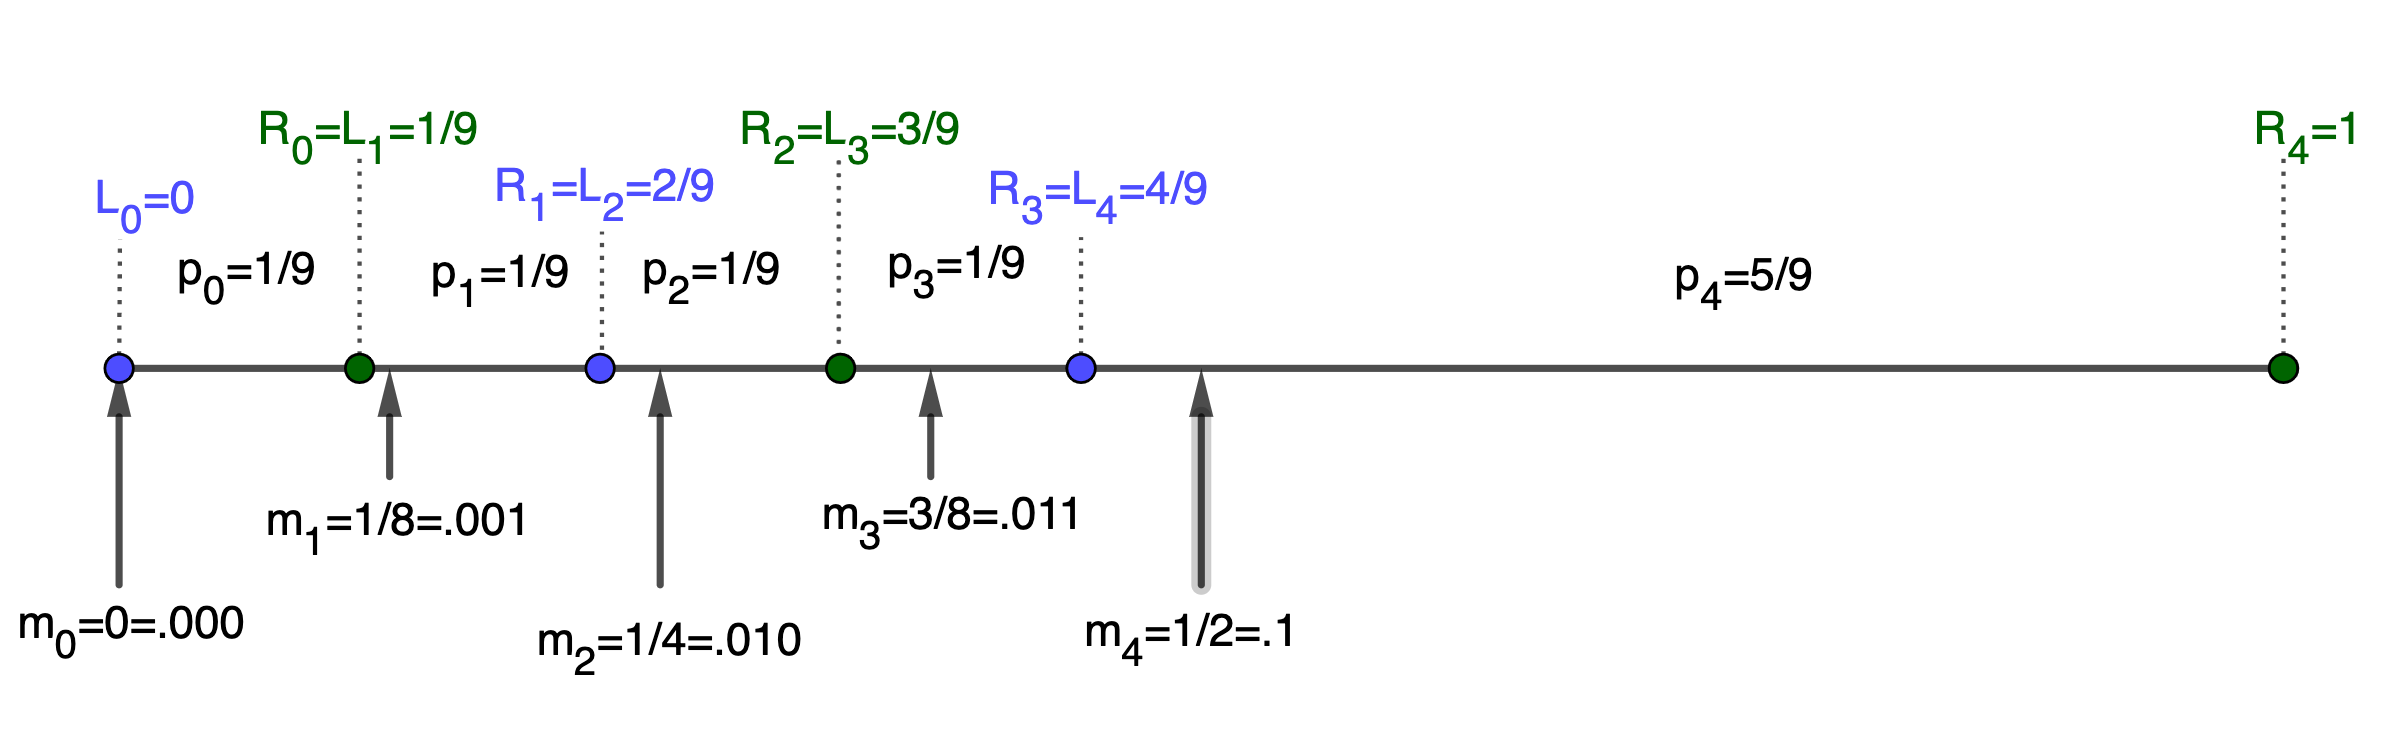
\includegraphics[width=1.0\textwidth]{Elias_Coding.png}
\end{figure}
\end{center}
\end{frame}


\begin{frame}{Elias coding: Codewords for prefix code}

\loud{Modification required for prefix code}
\bit
\item Code defined on last slides is \loud{not} always a prefix code.
\item For construction prefix code: 
\bit
\item Choose $l_i:=\lceil-\log_2(p_i)\rceil\mathbf{+1}$.
\item Choose $m_i$ as in \eqref{Propm},  but additionally require $m_i$ to be close to the midpoint of interval,  $|m_i-(L_i+(R_i-L_i)/2)|<2^{-l_i}$. 
\item Define uniquely decodable code as before.
\eit
\item Can be shown: Resulting code is a prefix code.
\item Average codeword length $\overline{\ell}$ of this prefix code satisfies $H(p)+1\leq \overline{\ell}\leq H(p)+2$. 
\eit
\end{frame}

\begin{frame}{Elias coding: Incremental encoding and decoding}
\loud{Main advantage of idea of Elias coding:}
\bit
\item Idea of Elias coding very useful if combined alphabet of a source $(X_1,\dots,X_N)$ is 
to be coded.
\item  Elias coding can enable \ALERT{incremental coding}: Need only \loud{conditional 
probabilites} $p_{X_i|X_{i-1},\dots,X_1}$.
\item\loud {Basic idea: } Choose symbol ordering on the combined alphabet so that intervals are nested.
\eit
\vspace{-0.2cm}
\loud{Interval nesting:}
\bit
\item Main idea can be explained using two random variables. General case analogous. 
\item Given two random variables $Y$ and $Z$ with alphabets $\mathcal{A}_Y=\{y_0,\dots,y_K\}$, $\mathcal{A}_Z=\{z_0,\dots,z_M\}$.
\item Define ordering on $\mathcal{A}_Y\times\mathcal{A}_Z$ by $(y_0,z_0)\leq (y_0,z_1)\leq\cdots\leq (y_0,z_M)\leq (y_1,z_0)\leq\cdots\leq (y_K,z_M)$.
\item Interval partitioning in Elias coding for this ordering: 
\bit
\item First define interval partitioning for $p_{Y}$. Get intervals $[L_i,R_i)$ of length $p_Y(y_i)$ as above. 
\item Then partition each interval $[L_i,R_i)$ into intervals $[L_{i,j},R_{i,j})$ of length  $p_{Y,Z}(y_i, z_j)=p_{Z|Y}(z_j|y_i)p_Y(y_i)$.
\item One has $[L_{i,j},R_{i,j})\subseteq [L_i,R_i)$ for all $i$ and $j$. 
\eit
\item \textit{If} one has $[L_i,R_i)\subset [0,1/2)$, then first bit of codewords for $(y_i,z_j)$
is zero for \textit{all} j. If $[L_i,R_i) \subseteq [1/2,1]$, first bit is always one. 
\item[\iarrow ] First bit of codewords for $(y_i,z_j)$ depends only on $y_i$ in such a case. 
\eit

\end{frame}

\begin{frame}{Elias coding: Incremental coding. Arithmetic coding. }
\loud{Incremental coding versus conditional coding as defined in last lecture}
\bit
\item Incremental (Elias) coding does \textit{not} mean that for a symbol sequence $(x_1,\dots,x_N)$, a codeword is 
produced after every $x_i$. 
\item Thus: Incremental coding \textit{not} the same as conditional (Huffman) coding defined in last lecture.
\item Example: Incremental Elias coding yields compression close to joint entropy also if each source $X_i$ is binary. Conditional Huffman coding can not compress a binary source. 
%\item In fact: In many applications, idea of Elias coding is applied to binary sources $X_i$. 
\item\loud{But:} Only conditional probabilities are used in incremental coding.
\item\loud{And:} For long sequences, first bits of a codeword for $(x_1,\dots,x_N)$ depend only on the first individual symbols $(x_1,\dots,x_M)$ where typically $M\ll N$.  
\eit
\ALERT{Arithmetic coding: } 
\bit
\item Finite precision realization of Elias coding. 
\item Core engine for the lossless coding component of modern video coding standards. 
\item Conditional probabilities of underlying complicated sources are approximated using simple  
models.
\item Although mathematically equivalent, using only modelled conditional probabilities is \textit{practially much easier} than using a modelled joint probability of underlying source.
%\item Incremental encoding and decoding is exploited in the underlying standard.   
\eit

\end{frame}


\section{Outlook: Arithmetic coding in modern video coding standards}


\begin{frame}
 \vspace{8.0ex}
\begin{center}
\begin{beamercolorbox}[sep=12pt,center]{part title}
\usebeamerfont{section title}\insertsection\par
\end{beamercolorbox}
\end{center}
\end{frame}


 \input{../../..//SS2020/slides/CoeffCoding/CABAC/BasicDesign/BasicDesign.tex}                  


\begin{frame}{Binary probabilities by exponentially moving averages}
\loud{Setup:} 
\bit
\item Consider discrete binary random variable $X(t)$, $t\in\mathbb{N}\cup\{0\}$. 
\item Let $P(t)$ be the probability of $1$ at time $t+1$. 
\eit
\loud{Definition of probability based on previous outcomes:}
\bit
\item Fix $P(-1)$ and for $t\geq 0$ set
\begin{align}\label{SlideWindowProb}
P(t)=(1-\sigma) P(t-1)+\sigma X(t), \qquad 0\leq \sigma\leq 1. 
\end{align}
\item Parameter $\sigma$ is called \loud{adaptation rate}.
\eit
\bit
\item By induction: Can write
\[
P(t)=\sum_{i=0}^{t}\sigma(1-\sigma)^iX(t-i)+(1-\sigma)^{t+1}P(-1). 
\] 
Second summand approaches $0$ as $t\to\infty$.
\item[\iarrow] $P(t)$ is a \loud{weighted sum} of the $X(t-i)$, $0\leq i\leq t$, weights \loud{decrease exponentially} in $i$ and sum of weights approaches one as $t\to\infty$.
\eit
\end{frame}

\begin{frame}{Representation of exponentially moving averages by state machine}
Represent probability $P(t)$ in terms of 
\bit
\item $P_{LPS}(t)\in (0,0.5]$, probability of \loud{least probable sympbol} at time $t+1$.
\item $\nu_{MPS}(t)\in\{0,1\}$, value of \loud{most probable symbol} at time $t$. 
\eit
Equation \eqref{SlideWindowProb} can then be rewritten as
\begin{align}\label{SlideWindowProbLPS}
P_{LPS}(t)=\begin{cases}\alpha\cdot P_{LPS}(t-1) & \text{, if $X(t)=\nu_{MPS}$} \\ 1-\alpha(1-P_{LPS}(t-1)) & \text{, if $X(t)\neq \nu_{MPS}$,}\end{cases}
\end{align}
where
$\alpha=1-\sigma$. 

In \loud{video coding standards H.264|AVC and H.265|HEVC}: 
\bit
\item Choose $\alpha \approx 0.95$. 
\item \loud{Logarithmic quantization} 
\begin{align}\label{Logquant}
P_{LPS}(t)=0.5\cdot \alpha^{S(t)},
\end{align}
$S(t)$ integral, $0\leq S(t)\leq 62$. 
\eit
\end{frame}

\begin{frame}{State transition rules for binary probability used in video codecs}
\begin{figure}
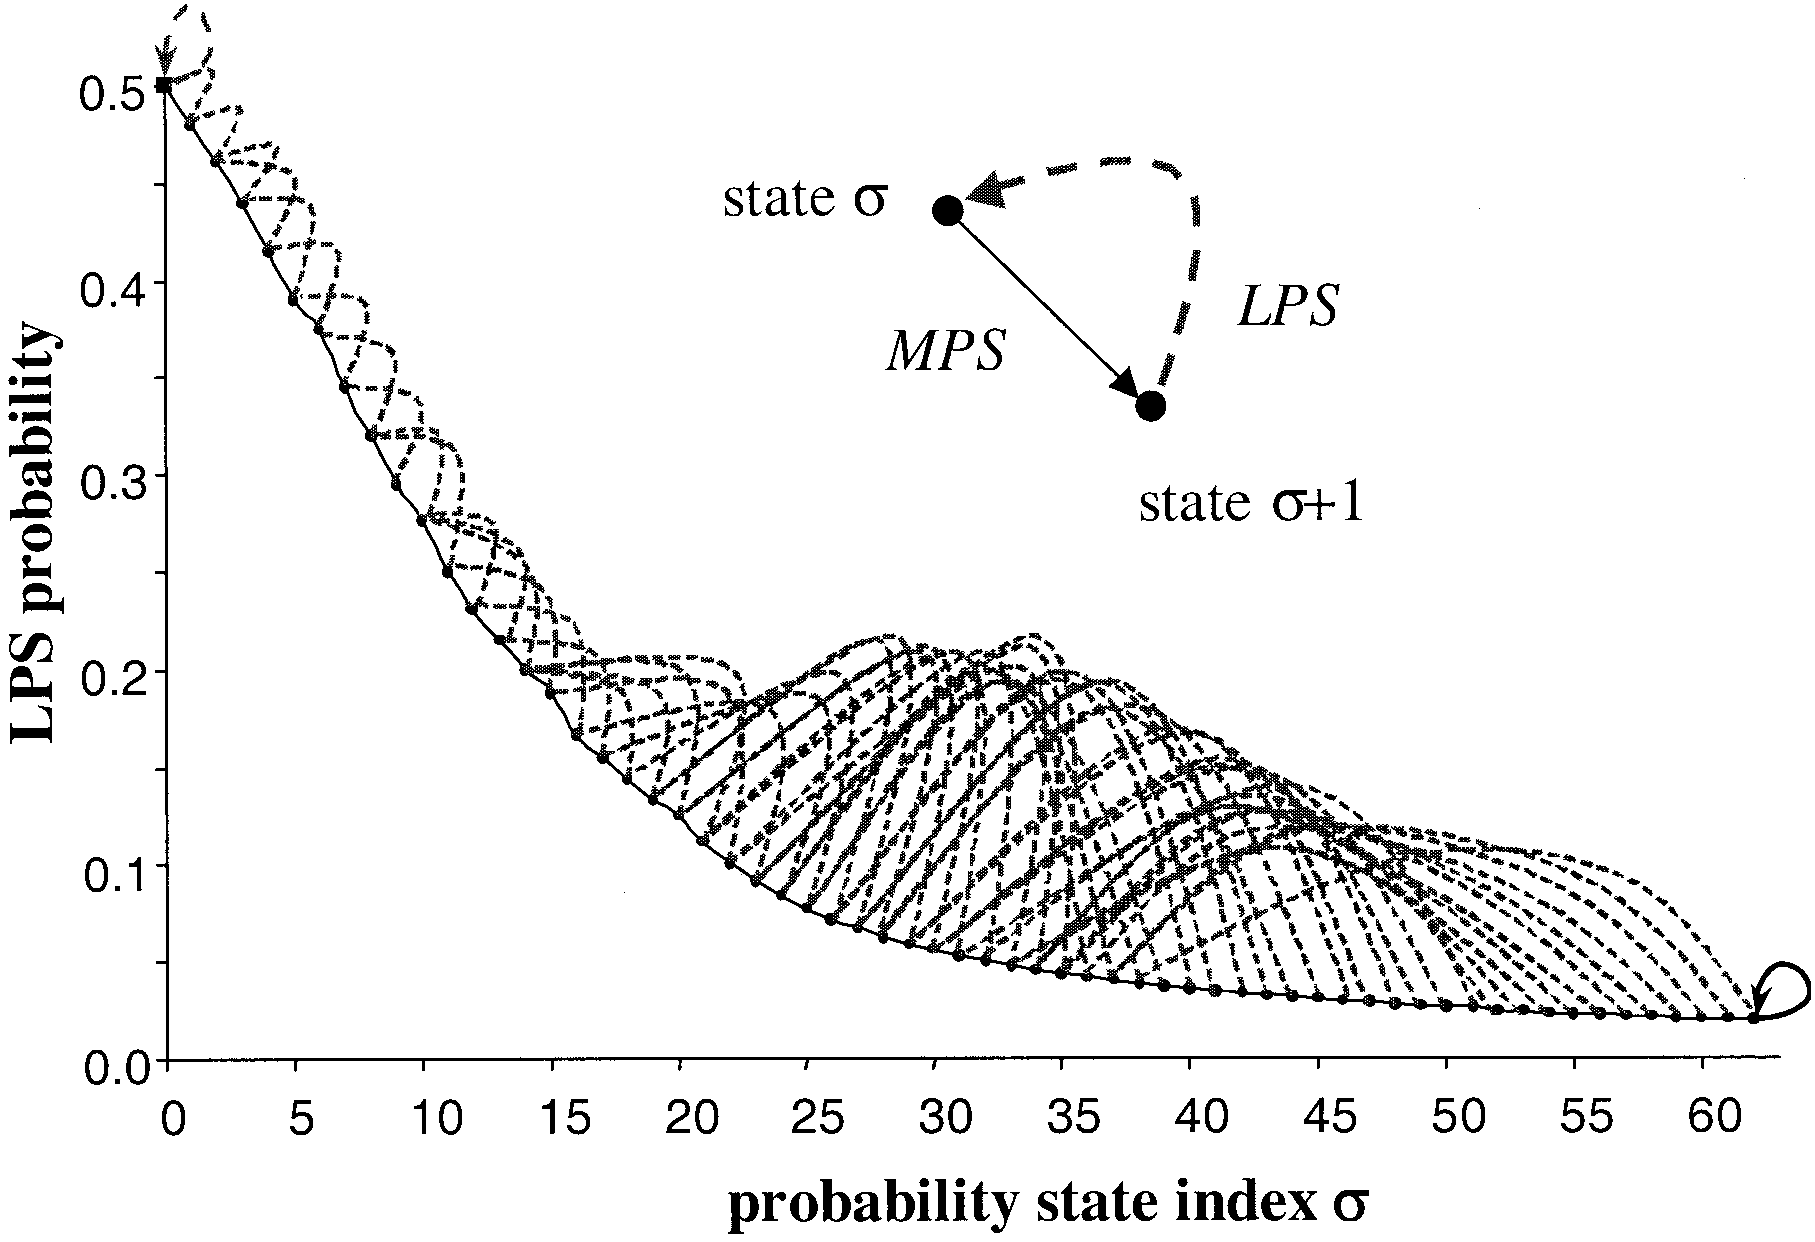
\includegraphics[width=.49\textwidth]{CabacStateTransition.png}
\captionsetup{labelformat=empty}
\caption{State transition rules that implement \eqref{SlideWindowProbLPS} and \eqref{Logquant}, taken from Marpe et al., 2003.}
\end{figure}

\end{frame}



\section{Rate-Distortion Theory I}


\begin{frame}
 \vspace{8.0ex}
\begin{center}
\begin{beamercolorbox}[sep=12pt,center]{part title}
\usebeamerfont{section title}\insertsection\par
\end{beamercolorbox}
\end{center}
\end{frame}

\subsection{Introduction}

\begin{frame}{Introduction}
Notation: Let $X$ be a discrete random variable with alphabet $\mathcal{A}:=\mathcal{A}_X$ and distribution $p:=p_X$.

\loud{Up to now: Lossless coding} 
\bit
\item Transmission that enables exact reconstruction of coded messages at the decoder.  
\item Rate, i.e. average expected codeword length, measures the quality of a lossless compression system. 
\eit
\loud{Now: Lossy source coding} 
\bit 
\item  To decrease the rate, allow that transmitted $x\in\mathcal{A}$ may not 
be exactly recoverd by a decoder. 
\item Allow \loud{distortion} between encoded and decoded $x$. 
%\item Dviation is described by a \loud{distortion} function, i.g.  squared Euclidean or Hamming distance. 
\item Only lossless transmission of quantization indices by a uniquely decodable code yielding a \loud{rate}. 
\item[\iarrow] \loud{Lossy source code:} Rigorous definition of such an encoding-decoding procedure. 
\eit
\ALERT{Rate-Distortion Theory: } Theoretical analysis of \textit{all} lossy source codes. Established by \loud{Shannon}.  
\bit
\item \loud{Goal of next lectures:} Explain and proof \loud{Fundamental Theorem of Lossy Source Coding}. Description 
of best rate-distortion tradeoffs possible.    
\item Treat discrete iid. case first. Extension to sources with memory and continuous sources later. 
\eit
\end{frame}

\subsection{Lossy source codes}
\begin{frame}{Lossy source codes: Definition}
\begin{definition}
A lossy source code $Q=(\alpha,\gamma,\beta)$ for $\mathcal{A}$ is given by
\bit
\item An \loud{encoder mapping} 
\[
\alpha: \mathcal{A}\to \mathcal{I}_K:=\{1,2,\cdots,K\}. 
\]
Mapping $\alpha$ is also called quantization and $\mathcal{I}_K$ is called set of quantization indices. 
\item A \loud{uniquely decodable code} 
\begin{align*}
\gamma: \mathcal{I}_K\to \mathcal{B}^{<\infty}, 
\end{align*}
where $\mathcal{B}^{<\infty}$ is the 
set of finite bit-sequecens. 
\item A \loud{decoder mapping}
\[
\beta: \mathcal{I}_K\to\widehat{\mathcal{A}},
\]
also called inverse quantization into a finite alphabet $\widehat{\mathcal{A}}$, called reproduction alphabet.
\eit
\end{definition}
Lossy source codes are the common setup for all compression systems studied in this lecture. 
\end{frame}

\begin{frame}{Lossy source codes: Basic properties}
\loud{Transmission of a symbols $x\in\mathcal{A}$ by a lossy source code}
\bit
\item Encoder computes  $\mathsf{i}=\alpha(x)$ and converts it to a bit sequence $\mathsf{b}=\gamma(\mathsf(i))$. 
\item Bit sequence $\mathsf{b}$ is transmitted to the decoder. 
\item Decoder recovers $\mathsf{i}=\gamma^{-1}(\mathsf{b})$ and computes the reconstructed value 
$\hat{x}\in\mathbb{R}^N$ as 
\begin{align*}
\hat{x}=\beta(\mathsf{i})=\beta(\alpha(x)).
\end{align*} 
\item In general one has $\hat{x}\neq x$, i.e. the source code is lossy.  
\item Deviation of $\hat{x}$ from $x$ is quantified by a distortion function. 
\eit
\begin{center}
\tikzstyle{encdec} = [rectangle, rounded corners, minimum width=2cm, minimum height=1cm,text centered, align=center, text width=1.9cm, draw=black]
\tikzstyle{iomsg} = [rectangle, rounded corners, minimum width=2cm, minimum height=1cm,text centered, text width=1.5cm, draw=black, fill=red!30]
\tikzstyle{iomsgN} = [rectangle, rounded corners, minimum width=2cm, minimum height=1cm,text centered, text width=1.5cm, draw=black, fill=green!30]
\tikzstyle{arrow} = [thick,->,>=stealth]
\begin{tikzpicture}[node distance=2cm]
\node (inmsg) [iomsg] {Input\\ x};
\node (quant) [encdec, right of = inmsg, xshift=0.5cm ] {Quantization:\\ $\mathsf{i}=\alpha(x)$};
\node (enc) [encdec, right of = quant, xshift=0.5cm ] {Lossless:\\ $\mathsf{b}=\gamma(\mathsf{i})$};
\node (dec) [encdec, right of = enc, xshift=2.0cm ] {Lossless:\\ $\mathsf{i}=\gamma^{-1}(\mathsf{b})$};
\node (outmsg) [iomsgN, right of = dec, xshift=0.5cm ] {Output\\ $\hat{x}=\beta(i)$};
\draw [arrow] (enc) -- node[anchor=south] {bit-stream $\mathbf{b}$} (dec);
\draw [arrow] (enc) -- node[anchor=north] {$\mathbf{b}=00101$} (dec);
\draw [arrow] (inmsg) -- (quant);
\draw [arrow] (quant) -- (enc);
\draw [arrow] (dec) -- (outmsg);
\end{tikzpicture}
\end{center}
\end{frame}

\subsection{Rate distortion function}
\begin{frame}{Distortion function}
\bit
\item A distortion function $d$ is a mapping
\begin{align*}
d: \mathbb{R}\times\mathbb{R}\to [0,\infty), \qquad \text {with $d(x,x')=0$ if and only if $x=x'$}.
\end{align*}
%meant to measure the distance from $x$ to $x'$. 
\item \loud{Squared Euclidean distance} 
\begin{align*}
d(x,x')=(x-x')^2.
\end{align*}
\item \loud{Hamming distance}
\begin{align*}
d(x,x')=\begin{cases} 0 & \text{if $x\neq x'$} \\ 1 & \text{else.}  \end{cases}
\end{align*}
\item \loud{Additive extension:} of $d$ to a distortion function $d_N$ on $\mathbb{R}^N$ by   
\[
d_N:\mathbb{R}^N\times\mathbb{R}^N\to [0,\infty),\quad d_N((x_1,\dots,x_N),(x_1',\dots,x_N')):=\frac{1}{N}\sum_{i=1}^Nd(x_i,x_i'). 
\]
\eit 
\end{frame}

\begin{frame}{Rate and distortion of a source code}
\begin{definition}
Let $Q=(\alpha,\gamma,\beta)$ be a source code for $\mathcal{A}$ 
and fix a distortion function $d$. 
\bit
\item Rate $r(Q)$: Expected number of bits for transmitting 
quantized source symbols $\alpha(x)$ 
by $\gamma$:  
\begin{align*}
r(Q)=\sum_{x\in\mathcal{A}}p(x)\ell(\gamma(\alpha(x))),
\end{align*}
where $\ell(\gamma(x))$ denotes the lenght of the codeword $\gamma(x)$. 
\item Distortion $\delta(Q)$: Expected distortion between reconstructed and original symbols:
\[
\delta(Q)=\sum_{x\in\mathcal{A}}p(x)d(x,\beta(\alpha(x))). 
\]
\eit 
\end{definition}
\loud{Relation to previous lectures:}
\bit
\item Rate is the \loud{average codeword-length} of $\gamma$, where $\mathcal{I}_K$ is equipped with pmf induced by $\alpha$ and $p$. 
%\[
%r(Q)=\sum_{i\in\mathcal{I}_K}\bigl(\sum_{x\in\mathcal{A}\colon \gamma(x)=i}p(x)\bigr)\ell(\gamma(i)). 
%\]
\item Distortion was not present in previous lectures.
\eit  
\end{frame}


\begin{frame}{Rate distortion function}
\ALERT{Goal of designing source codes:} 
\bit
\item[]For a given maximum distortion $D$, find a source code $Q$ of distortion $\delta(Q)\leq D$ that minimizes the rate $r(Q)$ among 
all source codes whose distortion does not exceed $D$.
\eit 

\ALERT{\iarrow $ $ Rate-distortion function: } 
\bit
\item[] Describe optimal performance that can be achieved at all up to an arbitrary small deviation for the above task.
More formally: For $D\in[0,\infty)$, one defines
\begin{equation*}
\boxed{R(D):= \inf\{r(Q)\colon \text{Q is a source code with } \delta(Q)\leq D \}.} 
\end{equation*}
\eit 

\ALERT{Rate-distortion theory: } 
\bit
\item[] Study rate distortion function of a given source. Derive theoretical performance limits for all lossy compression systems one wants to build. 
\eit 

  

\end{frame}


\begin{frame}{Rate distortion function: Elementary properties}
\bit
\item R(D) is a monotonically decreasing function of $D$.  Reason: If $D_1\geq D_2$, then $R(D_1)$ is infimum over a larger 
set than $R(D_2)$.

\item Since $\mathcal{A}$ is finite: $D=0$ is possible. $R(D)$ coincides with the optimal average codeword length for coding $\mathcal{A}$. 
%\item[\iarrow] Huffmann coding: Explicit method to construct source code that realizes $R(0)$. %In particular: Explicit computation of $R(0)$.
\item There exists a $D_{max}\in (0,\infty)$ such that $R(D)=0$ for all $D\geq D_{max}$ and such that $R(D)>0$ for all $D<D_{max}$. 
\item Case of squared Euclidean distance: $D_{max}$ is equal to the variance of the source. 
\eit

\begin{center}
\begin{figure}
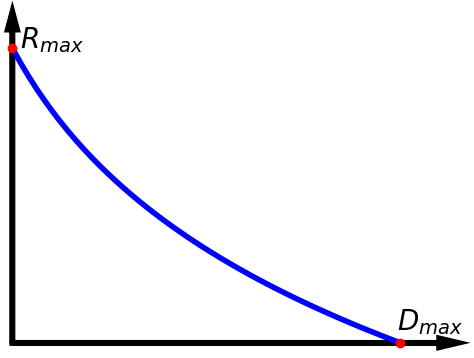
\includegraphics[width=0.25\textwidth]{RD_Plot_Final.png}
\captionsetup{labelformat=empty}
\caption{Example of a rate distortion function.}
\end{figure}
\end{center}

\end{frame}





%\begin{frame}{Passing to discrete iid. random processes} 
%Let $X$ be a random variable. \loud{Setup:} Not study source coding of $X$ alone, but joint coding of $N$ independent versions of $X$.
%
%\loud{Discrete iid process:}
%\bit
%\item A discrete random process $\mathcal{X}=(X_i)_{i=1}^{\infty}$ is called independent identically distributed (iid) with distribution $p_X$ if 
%\bit 
%\item All marginal distributions $p_{X_i}$ satisfy $p_{X_i}=p_X$.
%\item For each $i$ and each $T$, all random variables $X_{i},\dots,X_{i+T}$ are independent.
%\eit 
%\item Notations: Write 
%\begin{align*}
%X^N:=(X_1,\dots,X_N); \quad p^{\times N}:=p_{X^N},\quad  p^{\times N}(x_1,\dots,x_N)=p_X(x_1)\cdots p_X(x_N)
%\end{align*}    
%\item For the joint entropies, one has 
%\begin{align*}
%H(X^N)=\sum_{i=1}^NH(X). 
%\end{align*}
%\eit
%\end{frame}
\subsection{Extension to random processes}
\begin{frame}{Source code for $N$ realizations of a random variable} 
\loud{Setup:} Study joint coding of $N$ independent realizations of a random variable. .
\bit
\item For a random variable $X$, write 
\begin{align*}
X^N:=(X,\dots,X); \quad p^{\times N}:=p_{X^N},\quad  p^{\times N}(x_1,\dots,x_N)=p_X(x_1)\cdots p_X(x_N)
\end{align*}
\item $X^N$ is an $\mathbb{R}^N$-valued random-variable.  
\item Definition of source code $Q_N=(\alpha_N,\gamma,\beta_N)$  for $X^N$ is as before.
\bit
\item Encoder mapping $\alpha_N:\mathcal{A}^N\to \mathcal{I}_{K'}$.
\item Uniquely decodable code $\gamma_N$ on $\mathcal{I}_{K'}'$.
\item Decoder mapping $\beta_N:\mathcal{I}_{K'}'\to\mathcal{A}^N$. 
\eit
\item Rate $r(Q_N)$  and distortion $\delta(Q_N)$ of $Q_N$ are measured per symbol: 
\begin{align*}
r(Q_N)=1/N\sum_{x\in\mathcal{A}^N}p^{\times N}(x)\ell(\gamma_N(\alpha_N(x))), \quad \delta(Q_N)= 1/N\sum_{x\in\mathcal{A}^N}p^{\times N}(x)d(x,\beta_N(\alpha_N(x))).
\end{align*} 
\item[\iarrow] Rate distortion function for $X^N$ defined as above. 
\eit
\end{frame}


\begin{frame}{Joint coding needed even for iid souces} 
\loud{Joint coding important for optimality} 
\bit
\item A typical source code for $X^N$ is \loud{not} necessarily comprised by the concatenation of $N$ 
source codes for the indiviudal $X_i$, i.e. $N$ source codes of $X$, \loud{although} the $X_i$ are indpendent.
\item In fact:  For optimal source codes, one cannot expect this to be true. 
\eit
\vspace{-3.5mm}
\loud{Example from lossless case:}
\bit
\item  Assume that $X$ is any random variable such that $p_X(a)\neq 2^{-m}$, $m\in\mathbb{N}$, for an $a\in\mathcal{A}$. 
\item We know: Huffman code $\gamma$ for $X$ is optimal, \loud{but}
$\overline{\ell}(\gamma)=H(X)+\epsilon$ with an $\epsilon>0$.
\item Thus: Coding $X^N$ by coding each $X_i$ with $\gamma$  gives average codeword length $H(X)+\epsilon$ per symbol..    
\item On the other hand: Average codeword length per symbol of a joint  Huffman code for $X^N$
can be bounded by $1/N(H(X^N)+1)=H(X)+1/N$. 
\item[\iarrow] Thus: Joint coding is better than marginal coding even for iid sources. 
\eit
\vspace{-2.5mm}
\loud{Joint coding even much more important and helpful in lossy case:}
\bit
\item Only joint coding, i.e. \loud{vector quantization} exploits the \loud{space filling advantage}
\item Will be treated later. 
\eit
\end{frame}

\subsection{Mutual information and informational rate distortion function}

\begin{frame}{Mutual information for two random variables}
Let $X$ and $Y$ be discrete random variables with alphabets $\mathcal{A}_X$ and $\mathcal{A}_Y$.

\loud{Mutual information $I(X;Y)$:} 
\bit
\item Reduction of uncertainty of $X$ after observing $Y$: 
\item[\iarrow] Entropy as measure for uncertainty: 
\begin{align}\label{DefMutInf}
I(X;Y):=H(X)-H(X|Y). 
\end{align}  
\item In terms of the probability mass functions, one has 
\begin{align*}
I(X;Y)=\sum_{x\in\mathcal{A}_X}\sum_{y\in\mathcal{A}_Y}p_{X,Y}(x,y)\log_2\left(\frac{p_{X,Y}(x,y)}{p_{X}(x)p_{Y}(y)}\right). 
\end{align*}
\item[\iarrow] Mutual information is symmetric:
\[
I(X;Y)=I(Y;X).
\]
\item[\iarrow]  Applying Divergence Inequality: Mutual information is zero if and only if $X$ and $Y$ are independent. 
\eit
\end{frame}
\begin{frame}{Mutual information for conditional probability mass functions:} 
\loud{Mutual information can be defined given a marginal and a conditional distribution} 
\bit
\item Let $p$ be a pmf with finite alphabet $\mathcal{A}$. 
\item For some finite alphabet $\mathcal{B}$, let a conditional probabibility mass function $q(\cdot|x)$ on $\mathcal{A}$ be given. 
\item This means: $q(\cdot|x)$ is a probability mass function on $\mathcal{B}$ for 
each $x\in\mathcal{A}$. 
\item The pmf $p$ and the conditonal pmf $q$ define the probability masses $p(x)q(\hat{x}|x)$ of a joint distribution on $\mathcal{A}\times\mathcal{B}$.
\item[\iarrow] Thus: According to \eqref{DefMutInf}, one defines
\begin{align*}
I(p;q)=H(p)-H(q|p)=\sum_{x\in\mathcal{A}}\sum_{\hat{x}\in\mathcal{B}}p(x)q(\hat{x}|x)\log_2\left(\frac{q(\hat{x}|x)}{p(x)}\right).
\end{align*}
\item Definitions are consistent: For two random variables $X$ and $Y$, one has
\begin{align*}
I(X;Y)=I(p_X;p_Y). 
\end{align*}
\eit 
\end{frame}

\begin{frame}{The informational rate distortion function}
\begin{definition}
Let $\mathcal{A}$ be a finite source with pmf $p$. 
The informational rate-distortion function is defined as 
\begin{align}\label{DefInfRDRProb}
R^{(I)}(D):=\inf\{I(p;q)\colon \sum_{x\in\mathcal{A}}\sum_{\hat{x}\in\mathcal{B}}q(\hat{x}|x)p(x)d(x,\hat{x})\leq D\}
\end{align}
where $q$ is taken over the set of all conditional probabilities $q(\cdot|x)$ with finite alphabet $\mathcal{B}$.
\end{definition}
\ALERT{Main result: Informational rate distortion function can be used to describe rate distortion function of source coding.} 

\loud{\iarrow$ $ Advantage: } Function $R^{(I)}$ and analog for continuous sources is easier to study than rate distortion function.
%\begin{itemize}
%\item \loud{Main result: } Informational rate distortion function can be used to compute rate distortion function. 
%\item \loud{\iarrow Advantage: } Function $R^{(I)}$ and continuous analog is easier to study than rate distortion function. 
%\item Example: It can be shown that $R^{(I)}$ is convex. Important property even of R-D functions ``appearing in practise''. 
%\item Function $R^{I}$ can even be computed explicity for Gaussian sources.
%\item Algorithm  
%\end{itemize}

\end{frame}

\begin{frame}{Conditional probabilities in the informational rate distortion function} 

\loud{Conditional probabilities q appearing in $R^{(I)}$: }
\bit 
\item A finite alphabet $\mathcal{B}$ of size $m=|\mathcal{B}|$ is given. 
\item For each $x\in\mathcal{A}$ a probability mass function $q(\cdot|x)$  on $\mathcal{B}$ is given. 
\item If  $n:=|\mathcal{A}|$, for the given $\mathcal{B}$, conditional probabilites  $q$ correspond to all real $n\times m$-matrices $Q=(q_{i,j})$ such that 
\bit
\item $0 \leq q_{i,j} \leq 1$, for all $i,j$. 
\item $\sum_{j=1}^mq_{i,j}=1$ for all $i\in\{1,\dots,n\}$. 
\eit
\item[\iarrow] Minimization of \eqref{DefInfRDRProb} for all $\mathcal{B}$ and all such $Q$ that additionally satisfy the distortion constraint.
\item Alphabet $\mathcal{B}$ can be chosen freely, i.e. infimum over all possible $\mathcal{B}$ and $q$. 
\item Accordingly: Reproduction alphabets $\widehat{\mathcal{A}}$ of source codes can also be chosen freely.  
\item One can also fix a reproduction alphabet $\mathcal{B}$ both for the definition of all source codes and of informational rate-distortion function.  
\item Then: Infimum in \eqref{DefInfRDRProb}  is attained by some $q$, minimization of \eqref{DefInfRDRProb} is a convex optimization problem.
\item[\iarrow] \loud{Blahut-Arimoto algorithm: } Minimizing of \eqref{DefInfRDRProb} for fixed $\mathcal{B}$.  
\eit 
\end{frame}

\subsection{Fundamental theorem of lossy source coding}
\begin{frame}{Fundamental theorem of lossy source coding for discrete iid processes}
Main theorem of lossy source coding due to Shannon: 
\begin{theorem}[Fundamental theorem of lossy source coding]
Let $X$ be a discrete random variable. Fix an additive distortion measure. 
\begin{enumerate}
\item The informational rate distortion function $R^{I}$ is always a \loud{lower bound} for the rate distortion function: 
For every $N\in\mathbb{N}$ and every sorce code $Q_N$ for $X^N$ one has  
\begin{align}\label{BoundRate}
r(Q_N)\geq R^{(I)}(\delta(Q_N)). 
\end{align}
\item The bound \eqref{BoundRate} is \loud{asymptotically achievable}. For every $D\in[0,\infty)$ and every $\epsilon>0$, there exits an $N_0\in\mathbb{N}$ such that for each $N\geq N_0$, there 
exists a source code $Q_N$ for $X^N$ such that 
\begin{align*}
\delta(Q_N)\leq D+\epsilon
\end{align*}
and such that
\begin{align*}
r(Q_{N})\leq R^{(I)}(D). 
\end{align*}
\end{enumerate}
\end{theorem}
\end{frame}

%\begin{frame}{Fundamental theorem of lossy source coding: Outlook on the proof.}
%\loud{Outlook: Idea of proof of lower bound in fundamental lossy source coding theorem:}
%\bit
%\item Use \loud{convexity} of informational rate distortion function, see .. . 
%\item Use basic properties of entropy: \loud{Chain rule} and \loud{data processing inequalities}. 
%\eit 
%\loud{Outlook: Idea of the proof of asymptotic achievability: Random coding}
%\bit
%\item For each $N$ and $R'$, consider the set of all $\mathcal{A}^N$-valued sequences of length $2^{NR'}$.
%\item Each sequence defines a source code of rate $R'$.
%\item Set of sequences forms itself naturally a probability space, the \loud{ensemble set $\mathcal{E}$}.   
%\item Using \loud{theorem of large numbers}, show that for given rate $R'>R^{(I)}(D)$, expectation value of distortion on the ensemble 
%set is not greater than $D+\epsilon$ as $N\to \infty$.   
%\item To apply theorem of large numbers forces, one needs to consider $N\to\infty$ and not the single alphabet $\mathcal{A}$. 
%\item Consequence: there exists at least one sequence in $\mathcal{E}$ with distortion not larger than $D+\epsilon$. 
%\eit
%\item Details will be given in next lecture.
%\loud{Comments on the proof of asymptotic achievability: }
%\bit
%\item \loud{Proof is not constructive: } One only concludes that such a lossy code exists, no explicit construction. Different to lossless case: Huffman codes are defined explicitly.  
%\item Method of proof is similar to proof of \loud{Channel Coding Theorem}, although settings of source coding and channel coding are independent (Source-Channel-Separation Theorem). 
%\eit
%\end{frame}

\begin{frame}{Fundamental theorem of lossy source coding: Comments and outlook on the proof of lower bound.}

\bit
\item Statement and proof of above theorem, in particular asymptotic achievability, are \textit{not obvious at all}. 
\item Proof will be given in next lectures. 
\eit
\vspace{-2.5mm}
\loud{Application of fundamental theorem: Can describe rate distortion function for model sources}:
\bit
\item Example in the discrete case: Binary source. 
\item Continuous case: \loud{Gaussian sources}.
\item More general sources: \loud{Shannon lower bound}. 
\bit
\item Can estimate rate-distortion function from below. 
\item Estimate 
is \loud{asymptotically tight} for high rates or small distortions.  
\eit 
\eit 

\loud{Outlook: Idea of proof of lower bound in fundamental lossy source coding theorem:}
\bit
\item Use \loud{convexity} of informational rate distortion function. 
\item Use basic properties of entropy: \loud{Chain rule} and \loud{data processing inequalities}. 
\eit 
\end{frame}


\begin{frame}{Asymptotic achievabilty: Outlook on the proof. }
\loud{Outlook: Idea of the proof of asymptotic achievability: Random coding}
\bit
\item Let $q$ be a conditional probability on alphabet $\widehat{\mathcal{A}}$ close to the infimum in \eqref{DefInfRDRProb}.  
\item For each $N$ and $R'$, consider the set of all ${\widehat{\mathcal{A}}}^N$-valued sequences of length $2^{NR'}$.
\item Each sequence defines a source code of rate $R'$; all symbols coded with equal length. 
\item Set of sequences forms itself naturally a probability space, the \loud{ensemble set $\mathcal{E}$}.   
\item Using \loud{theorem of large numbers}, show that for given rate $R'>R^{(I)}(D)$, expectation value of distortion on the ensemble 
set is not greater than $D+\epsilon$ as $N\to \infty$.   
%\item To apply theorem of large numbers forces, one needs to consider $N\to\infty$ and not the single alphabet $\mathcal{A}$. 
\item Since expectation vaue not larger than $D+\epsilon$, there exists at least one sequence in $\mathcal{E}$ with distortion not larger than $D+\epsilon$. 
\eit
\loud{Comments on the proof of asymptotic achievability: }
\bit
\item \loud{Proof is not constructive: } One only concludes that such a lossy code exists, no explicit construction. Different to lossless case: Huffman codes are defined explicitly.  
\item Method of proof is similar to proof of \loud{Channel Coding Theorem}, although settings of source coding and channel coding are independent (Source-Channel-Separation Theorem). 
\eit 
\end{frame}


\subsection{Data processing inequalities}
\begin{frame}{Data processing inequalities: Statement}
%\loud{Definition:} 
\begin{definition}
Let $\mathbf{Z}$ be a discrete, $\mathbb{R}^n$-valued random variable. A discrete, $\mathbb{R}^m$-valued random variable \loud{$\mathbf{Y}$ determines $\mathbf{Z}$}, if $Z=\phi(\mathbf{Y})$ for 
a function $\phi:\mathbb{R}^m\to\mathbb{R}^n$.
\end{definition}
%\bit
%\item Let $\mathbf{Z}$ be a discrete, $\mathbb{R}^n$-valued random variable.
%\item \loud{Definition:} A discrete, $\mathbb{R}^m$-valued random variable \loud{$\mathbf{Y}$ determines $\mathbf{Z}$}, if $Z=\phi(\mathbf{Y})$ for 
%a function $\phi:\mathbb{R}^m\to\mathbb{R}^n$.
%\eit
\vspace{-2.5mm}

\loud{Heuristically:} If $\mathbf{Y}$ determines $\mathbf{Z}$:
\bit%\small
\item Knowing $\mathbf{Y}$, uncertainty about $\mathbf{Z}$ should be zero.
\item Uncertainty of $\mathbf{Z}$ should not be greater than uncertainty of $\mathbf{Y}$.
\item Knowing $\mathbf{Z}$ does not decrease the uncertainty ofanother random-variable $\mathbf{X}$ more than knowing $\mathbf{Y}$.    
\eit 
\loud{\iarrow Entropy as measure for uncertainty:}
\begin{proposition}[Data processing inequalities]
Let $\mathbf{Y}$ be a discrete, $\mathbb{R}^m$-valued random variable. Let 
$\phi:\mathbb{R}^m\to\mathbb{R}^n$ and let $\mathbf{Z}=\phi(\mathbf{Y})$. 
Then one has 
\begin{align*}
H(\mathbf{Z}|\mathbf{Y})=0 \qquad\text{and} \qquad H(\mathbf{Z})\leq H(\mathbf{Y}).  
\end{align*}
If $\mathbf{X}$ is another random variable, then 
$H(\mathbf{X}|\mathbf{Y})\leq H(\mathbf{X}|\mathbf{Z})$. 
\end{proposition}
\end{frame}

\begin{frame}{Data processing inequalities: Proof}
\bit 
\item One has $p_{Z|Y}(z|y)=1$ if $z=\phi(y)$ and $p_{Z|Y}(z|y)=0$, else. Thus 
$H(\mathbf{Z}|\mathbf{Y})=0$.
\item With chain rule for entropy, it follows that
\begin{align*}
H(\mathbf{Y})=H(\mathbf{Y})+H(\mathbf{Z}|\mathbf{Y})=H(\mathbf{Y},\mathbf{Z})=H(\mathbf{Z})+H(\mathbf{Y}|\mathbf{Z}).
\end{align*}
Since entropy is non-negative, it follows that $H(\mathbf{Y})\geq H(\mathbf{Z})$.
\item 
One has $p_{X,Y,Z}(x,y,z)=p_{X,Y}(x,y)$ if $z=\phi(y)$ and $p_{X,Y,Z}(x,y,z)=0$, else. 
\item For $z=\phi(y)$ and 
$p_Y(y)\neq 0$, one has $p_{X|Y,Z}(x|z,y)=p_{X|Y}(x,y)$. 
\item[\iarrow] This implies that $H(\mathbf{X}|\mathbf{Y})=H(\mathbf{X}|\mathbf{Y},\mathbf{Z})$.
\item Last lecture: $H(\mathbf{X}|\mathbf{Y},\mathbf{Z})\leq H(\mathbf{X}|\mathbf{Z})$ .
Thus $H(\mathbf{X}|\mathbf{Y})\leq H(\mathbf{X}|\mathbf{Z})$. \qed
\eit 
\end{frame}


\subsection{Convexity of the informational rate distortion function}
\begin{frame}{Review: Convexity and concavity}
\loud{Recall: Convexity of a function}
\bit
\item A function $f:(a,b)\to\mathbb{R}$ is called \loud{convex} if for any two point $p_1,\:p_2\in (a,b)$, the straight
line between $(p_1, f(p_1))$ and $(p_2, f(p_2))$ lies above the graph of $f$:
\begin{align}\label{eqconv}
f((1-\lambda)p_1+\lambda p_2)\leq (1-\lambda)f(p_1)+\lambda f(p_2), \quad \forall \lambda\in [0,1] 
\end{align}  
\item  $f$ is called \loud{strictly convex} if strict inequality holds in \eqref{eqconv} for all $\lambda\in (0,1)$ and 
all $p_1\neq p_2$. 
\item $f$ is calleld (strictly) \loud{concave}, if $-f$ is (strictly) convex. 
\eit
\begin{figure}
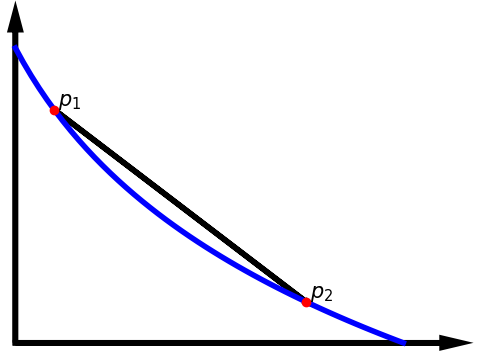
\includegraphics[width=0.26\textwidth]{RD_Plot_Convex_Final.png}
\captionsetup{labelformat=empty}
\caption{Illustration of convexity.}
\end{figure}
\end{frame}

\begin{frame}{Elementary properties of convex functions}
\loud{Jensen's inequality}
\bit
\item If $f$ is convex on $(a,b)$, then for all $\lambda_1,\dots,\lambda_n\in[0,1]$ with $\lambda_1+\dots+\lambda_n=1$ and all 
$p_1,\dots,p_n\in (a,b)$, one has
\begin{align*}
f(\lambda_1 p_1+\dots+\lambda_np_n)\leq \lambda_1f(p_1)+\dots+\lambda_nf(p_n). 
\end{align*}
\item If $f$ is strictly convex and all $p_i$ different, equality only if $\lambda_i=1$ for an $i\in\{1,\dots,n\}$. 
\item Proof by induction.
\eit
\loud{Characterization for continuously differentiable functions}
\bit
\item If $f$ is continously differentiable, then $f$ is (strictly) convex if and only if $f'$ is (strictly) monotonically increasing. 
\item Analogous statement for concave functions.  
\item Proof: Application of  mean value theorem of differential calculus.
\eit


\end{frame}

\begin{frame}{Concavity of entropy}
\begin{proposition}[Concavity of entropy]
Let $p_1$, $p_2$ be probability mass functions on a finite alphabet $\mathcal{A}$. 
Then for every $\lambda\in(0,1)$ one has 
\begin{align*}
H((1-\lambda)p_1+\lambda p_2)\geq (1-\lambda)H(p_1)+\lambda H(p_2), \quad \text{equality if an only if $p_1=p_2$}. 
\end{align*}
\end{proposition}
%\vspace{-0.1cm}
%\small Heuristic explanation: Averaging two pmfs gives a `more equidistributed pmf' $\iarrow$ entropy increases. 
\vspace{-2.9mm}
%\smallskip
\loud{Proof: } 
%\vspace{-1.5mm}
\bit 
\item Let $f(t):=-t\log_2(t)$. 
\item The derivative $f'(t)=-\frac{1}{\ln(2)}(1+\ln(t))$ is strictly decreasing $\loud\iarrow$ f is strictly concave. 
\item[\iarrow] By definition of the entropy:
\begin{align*}
H((1-\lambda)p_1+\lambda p_2)=\sum_{a\in\mathcal{A}}f((1-\lambda)p_1(a)+\lambda p_2(a))
\geq & \sum_{a\in\mathcal{A}}\left((1-\lambda)f(p_1(a))+\lambda f(p_2(a))\right)\\
=&(1-\lambda)H(p_1)+\lambda H(p_2).
\end{align*} 
 \item Statement of equality follows from strict concavity of $f$.  \qed
\eit
Heuristic explanation: Averaging two pmfs gives a `more equidistributed pmf' $\iarrow$ entropy increases. 
\end{frame}




\begin{frame}{Convexity of the informational rate distortion function}
\begin{proposition}[Convexity of $R^{(I)}$]
The informational rate distortion function $R^{(I)}$ is convex.
\end{proposition}
\vspace{-2.9mm}
\loud{Proof: } 
%\vspace{-1.0mm}
\bit
\item \loud{Main idea:} Use concavity of entropy, i.e. convexity of negative entropy. 
\item Let $\lambda\in [0,1]$ and $D_1,\:D_2\in[0,\infty)$. %One needs to show that
%\[
%R^{(I)}((1-\lambda)D_1+\lambda D_2)\leq (1-\lambda)R_I(D_1)+\lambda R(D_2). 
%\]
%
%
\item Let $q_1$ and $q_2$ be any conditinonal probabilities with alphabets $\mathcal{B}_1$ and $\mathcal{B}_2$ such that
\begin{align}\label{DistConstrIndiv}
\sum_{x\in\mathcal{A}}\sum_{\hat{x}\in\mathcal{B}_1}p(x)q_1(\hat{x}|x)d(x,\hat{x})<D_1; \quad \sum_{x\in\mathcal{A}}\sum_{\hat{x}\in\mathcal{B}_2}p(x)q_2(\hat{x}|x)d(x,\hat{x})<D_2.
\end{align}

\item Define a conditional probability $q_3$ with alphabet $\mathcal{B}=\mathcal{B}_1\cup\mathcal{B}_2$ as 
\begin{align*}
q_3=(1-\lambda)p_1+\lambda_2 p_2
\end{align*}
\item By \eqref{DistConstrIndiv}, $q_3$ satisfies the distortion constraint
\begin{align}\label{DistConstrQ3}
\sum_{x\in\mathcal{A}}p(x)\sum_{\hat{x}\in\mathcal{B}}q_3(\hat{x}|x)d(x,\hat{x}) \leq (1-\lambda)D_1+\lambda D_2. 
\end{align}
\eit
\end{frame}


\begin{frame}{Proof of the convexity of $R^{(I)}_X$}
\bit
\item By the concavity of entropy: 
\begin{align*}
-H(q_3|p)=-\sum_{x\in\mathcal{A}}p(x)H(q_3(\cdot|x))\leq& -\sum_{x\in\mathcal{A}}p(x)\left((1-\lambda)H(q_1(\cdot|x))+\lambda H(q_2(\cdot|x))\right)\\
=&-(1-\lambda)H(q_1|p)-\lambda H(q_2|p)
\end{align*}
\item [\iarrow] Using definition of $R^{(I)}$ and \eqref{DistConstrQ3}:
\begin{align}\label{estD}
R^{(I)}((1-\lambda)D_1+\lambda D_2)\leq I(p;q_3)=H(p)-H(p|q_3)\leq &(1-\lambda)H(p)+H(p|q_1)+\lambda( H(p)+H(p|q_2)) \nonumber\\ =&(1-\lambda)I(p;q_1)+\lambda I(p;q_2).
\end{align}
\item Now use:
\bit
\item $q_1$ and $q_2$ were arbitrary conditional probabilities satisfying \eqref{DistConstrIndiv}. 
\item Infimum of linear combinations is linear combination of infima. 
\item Infimum is largest lower bound. 
\eit
\item[\iarrow] It follows from \eqref{estD} that
\begin{align*}
R^{(I)}((1-\lambda)D_1+\lambda D_2)\leq (1-\lambda)R^{(I)}(D_1)+\lambda R^{(I)}(D_2). 
\end{align*}
\qed
\eit 
\end{frame}


%\begin{frame}{Estimate of rate by mutual informations}
%\begin{proposition}[Estimate of rate by mutual informations]
%Let a length n source code $(f_n,g_n)$ of rate $R$ be given.  Then one has 
%\begin{align}\label{EqRate}
%R\geq \sum_{i=1}^{n}I(X_i,Y_i) 
%\end{align}
%\end{proposition}
%Proof of the converse statement:
%\bit 
%\item The encoder needs to transmit $f(\mathbf{X}))$. \loud{Entropy is lower bound for rate \iarrow}
%\begin{align*}
%R\geq H(f(\mathbf{X})).
%\end{align*}
%\item Since $f(\mathbf{X})$ determines $Y=g(f(\mathbf{X}))$, one has 
%\begin{align*}
%H(f(\mathbf{X}))\geq H(\mathbf{Y})
%\end{align*}
%by ... . 
%\item Since $\mathbf{X}$ determines $\mathbf{Y}$, one has $H(\mathbf{Y}|\mathbf{X})=0$. Using the symmetry of $I$, it follows that
%\begin{align*}
%H(\mathbf{Y})=I(\mathbf{Y},\mathbf{X})=I(\mathbf{Y};\mathbf{Z})=H(\mathbf{X})-H(\mathbf{X}|\mathbf{Y}).
%\end{align*}
%
%\eit 
%Since $\mathbf{Y}$ determines $Y_i$ via the projection onto the $i$-th coordinate, it follows that
%\begin{align*}
%H(X_i|\mathbf{Y})\leq H(\mathbf{X}|Y_i). 
%\end{align*}
%By the chain rule, one has 
%\begin{align*}
%H(\mathbf{X}|Y_i)=\sum_
%\end{align*}
%\end{frame}
%\begin{frame}{Estimate of rate by mutual informations}
%\bit
%\item Since $\mathbf{X}$ is iid, $X_i\sim X$, one has
%\begin{align*}
%H(\mathbf{X})=\sum_{i=1}^nH(X_i)
%\end{align*}
%\item By the chain-rule, one has
%\begin{align*}
%H(\mathbf{X}|\mathbf{Y})=\sum_{i=1}^NH(X_i|\mathbf{Y},X_1,\dots,X_i).
%\end{align*}
%\item Since $(\mathbf{Y},X_1,\dots,X_i)$ determines $Y_i$ (or since ``conditioniong does not increase entropy'') one has
%\begin{align*}
%H(X_i|\mathbf{Y},X_1,\dots,X_i)\leq H(X_i|Y_i).  
%\end{align*}
%\item Combining the chain of inequlities gives 
%\begin{align*}
%R\geq \sum_{i=1}^nH(X_i)-H(X_i|Y_i)=\sum_{i=1}^nI(X_i|Y_i). \qed
%\end{align*}
%\eit 
%\end{frame}
%
%\begin{frame}
%\bit 
%\item \loud{Idea: Use convexity of $R^{(I)}$ and previous proposition}.
%\item \loud{Property of joint distributions $p_{X_i,Y_i}$}: 
%
%For all $x,\hat{x}\in\mathcal{A}$ and all $i\in\{1,\dots,N\}$,  $p_{X_i,Y_i}(x,\hat{x})$ is equal to the probability $p^{\times N}$ 
%of all $\mathbf{x}=(x_1,\dots, x_{i-1},x_i,x_{i+1},\dots,x_N)\in\mathcal{A}^N$ 
%with $x_i=x$ and $g_i(f(\mathbf{x}))=\hat{x}$. 
%\item Consequece: One has
%\begin{align*}
%D_i:=\sum_{x\in\mathcal{A}}\sum_{\hat{x}\in\mathcal{A}}p_{X_i,Y_i}(x,\hat{x})d(x,\hat{x})
%%=&\sum_{x\in\mathcal{A}}\sum_{\hat{x}\in\mathcal{A}}p_{Y_i|X_i}(\hat{x}|x)d(x,\hat{x})\\
%%\]
%%\item It easily follows from the definition that
%%then 
%%\[
%%D_i
%=&\sum_{\mathbf{x}=(x_1,\dots,x_N)\in\mathcal{A}^N}p^{\times N}(\mathbf{x})d(x_i,g_i(f(\mathbf{x}))).
%\end{align*}
%\item Thus, using ..., it follows that 
%\begin{align*}
%D=\sum_{\mathbf{x}\in\mathcal{A}^N}p^{\times N}(\mathbf{x})d_N(\mathbf{x},\mathbf{Y}(\mathbf{x}))
%=&\sum_{\mathbf{x}=(x_1,\dots,x_N)\in\mathcal{A}^N}p^{\times N}(\mathbf{x})(d(x_1,Y_1(\mathbf{x}))+\cdots+d(x_N,Y_N(\mathbf{x}))
%\\=&\sum_{i=1}^N D_i.
%\end{align*}
%\item[\iarrow] Using \eqref{EqRate} and the convexity of $R^{(I)}$, it follows that
%\begin{align*}
%R\geq \sum_{i=1}^NI(X_i;Y_i)\geq \sum_{i=1}^NR^{(I)}(D_i)\geq R^{I}(D)\qed 
%\end{align*}
%\eit
%\end{frame}






\end{document}